% standard
\documentclass[a4paper,11pt]{article}
\usepackage[utf8]{inputenc}
\usepackage[ngerman]{babel}

\usepackage{titlesec}
\usepackage{tocbibind}
\renewcommand{\listoffigures}{\begingroup
\tocsection
\tocfile{\listfigurename}{lof}
\endgroup}

\setcounter{secnumdepth}{5}
\setcounter{tocdepth}{5}
\titleformat{\paragraph} {\normalfont\normalsize\bfseries}{\theparagraph}{1em}{}
\titlespacing*{\paragraph}
{0pt}{3.25ex plus 1ex minus .2ex}{1.5ex plus .2ex}

%for linkt page numbers in table of content
\usepackage[linktocpage=true]{hyperref}

\hypersetup{%
unicode,pdffitwindow,
pdfkeywords = {pdf, LaTeX, hyperref, thumbnails}, 
pdfauthor = {Brüder Grimm},
bookmarksopen = true,
bookmarksnumbered = true,
pdfcenterwindow=true,
pdffitwindow = true,
pdfstartview=FitBV,
pdfcreator = {pdflatex},
colorlinks=true, breaklinks=true, %
urlcolor=magenta, % color for \url
filecolor=cyan, % color for file
linkcolor=black, % color for \ref
citecolor=magenta, %color for \cite
menucolor=darkblue,
breaklinks=true,anchorcolor=green
}

% for the Glossar, toc for table of Content visibility
\usepackage[toc]{glossaries}
\renewcommand*{\glstextformat}[1]{\textcolor{blue}{#1}}


% geometry
\usepackage{geometry}
\geometry{ headsep=20pt,
headheight=20pt,
left=21mm,
top=15mm,
right=21mm,
bottom=15mm,
footskip=20pt,
includeheadfoot}

% for using wrapfigures
\usepackage{wrapfig}

% header and footer
\usepackage{datetime}
\newdateformat{dmy}{%
\THEDAY.~\monthname[\THEMONTH] \THEYEAR}
\usepackage{fancyhdr}
\pagestyle{fancy}
\lhead{Noah Vogt \& Simon Hammer}
\chead{}
%\rhead{\dmy\today}
\lfoot{}
\cfoot{Gymnasium Kirschgarten}
\rfoot{Seite \thepage}
\renewcommand{\footrulewidth}{.4pt}

% fix figure positioning
\usepackage{float}

% larger inner table margin
\renewcommand{\arraystretch}{1.4}

% no paragraph indent
\setlength{\parindent}{0em}

%for longer comments
\usepackage{comment}

%for appendix
\usepackage[toc, page]{appendix}
\renewcommand\appendixpagename{Anhang}
\renewcommand\appendixtocname{Anhang}


%for spacing
\usepackage{setspace}
%\renewcommand{\baselinestretch}{1.5}
%\onehalfspacing
\linespread{1.25}

% graphics package
\usepackage{graphicx}

\usepackage{multicol}

\usepackage{multirow}

% use sans serif font
\usepackage{tgheros}
\usepackage{mathptmx}

% don't even ask what this is for, I have no idea (noah)
\usepackage{bm} %italic \bm{\mathit{•}}
\usepackage[hang]{footmisc}
\usepackage{siunitx}
\usepackage[font={small,it}]{caption}
\sisetup{locale = DE, per-mode = fraction, separate-uncertainty,   exponent-to-prefix, prefixes-as-symbols = false, scientific-notation=false
}
\newcommand{\ns}[4]{(\num[scientific-notation=false]{#1}\pm\num[scientific-notation=false]{#2})\cdot\num[]{e#3}\si{#4}}

% show isbn in bibliography
% \usepackage{natbib}

% for quotes
\newenvironment{nicequote}[2]{
    \begin{center}\begin{quote}\textit{#1}\\\par\raggedleft--- {#2}
    }{
    \end{quote}\end{center}
}

\makeindex

% using \say{} for easier quoting
\usepackage{dirtytalk}

% for code snippits
\usepackage{listings}
\usepackage{color}

\definecolor{dkgreen}{rgb}{0,0.6,0}
\definecolor{gray}{rgb}{0.5,0.5,0.5}
\definecolor{mauve}{rgb}{0.58,0,0.82}
\definecolor{background}{rgb}{0.36,0.36,0.36}

\lstset{
    numbersep=3pt,
    keywordstyle=\color{blue},
    commentstyle=\color{dkgreen},
    stringstyle=\color{mauve},
    breaklines=true,
    numbers=left,
    numberstyle=\scriptsize\color{black},
    frame=none,
    basicstyle = \small\ttfamily,
    breaklines=true
    breakatwhitespace=false,
    columns=flexible,
    xleftmargin=0.5cm,framesep=8pt,framerule=0pt,
    aboveskip=3mm,
    belowskip=3mm,
}

%\usepackage[backend=biber,style=apa]{biblatex}
\usepackage[
backend=biber,
style=alphabetic,
sorting=ynt,
]{biblatex}
\addbibresource{lit/refs.bib}

%========================Glossaries======================



\makeglossaries
% make glossary show up in toc
\renewcommand*{\glossarysection}[2][]{\section{#1}}

\newglossaryentry{copyleft}{
    name=Copyleft-Softwarelizenzen,
    description={Wie bei permissiven Lizenzen können Sie das Programm für JEDEN Zweck ausführen, den Quellcode lesen, ändern und die Änderungen veröffentlichen. Der Trick liegt jedoch in den restriktiven Redistributionsbedingungen: Sie dürfen das Programm NUR verbreiten, wenn Ihre Version die gleichen Freiheiten bietet. Dies geschieht in der Regel dadurch, dass die Weitergabe nur unter der gleichen Lizenz erlaubt ist. Der Name ``copyleft'' ist eine offensichtliche Anspielung auf das Wort ``Copyright'', da es versucht, dessen Konzept genau umzukehren: Anstatt die nahezu weltweit vorhandenen Kopierrechtsgesetze dazu zu verwenden, Nutzerfreiheiten einzuschränken, werden Copyleft-Lizenzen dazu eingesetzt, diese zu bewahren und zu erweitern. \cite{kumar2011}}
}

\newglossaryentry{permissive}{
    name=Permissive Softwarelizenzen,
    description={Mit diesen Lizenzen hat man das Recht das Programm für JEDEN Zweck zu benutzen, den Source Code zu lesen, ändern und seine Änderungen zu veröffentlichen. Ihr Name kommt von der Tatsache, dass sie ``permissiv'' sind, wenn es um ihre wenigen Einschränkungen geht: Sie schränken die Verbreitung des Quellcodes nicht sehr stark ein und erlauben es oft, die Software unter JEGLICHEN Bedingungen weiterzugeben. Das bedeutet, es ist möglich, den Fork eines permissiv lizenzierten Programms proprietär zu machen. Das bedeutet, dass Sie den Code nicht davor schützen, in anderen Projekten, selbst wenn diese proprietär sind, verwendet zu werden, ohne etwas zurück geben zu müssen. Das ist ein eindeutiger Nachteil und der Grund, warum manche Leute - meist auf Imageboards \cite{8chan.moe} - diese Lizenzen als ``Cuck Licenses'' beschimpfen, sie werden auch reichlich kritisiert auf diversen technologiebezogenen Blogposts\cite{cuckblog}.}
}

\newglossaryentry{fsf}{
    name=Free Software Foundation,
    description={dt. \say{Stiftung für freie Software}, ist eine von Richard Stallman\cite{rms} gegründete Stiftung, ursprünglich mit dem Ziel die Entwicklung des GNU Projekts zu finanzieren, was mittlerweile erweitert und erstetzt wurde durch die allgemeine Förderung und Entwicklung von \glspl{freie Software}.}
}

\newglossaryentry{freie Software}{
    name=Freie Software,
    plural=freier Software,
    description={engl. \say{free software}, ist nach der Definition der \gls{fsf} Software, welche die vier von ihnen definierten Grundfreiheiten garantiert: Das Verwenden der Software für jeden Zweck (keine willkürlichen, z.B. geografischen Einschränkungen etc.), der Quellcode darf ohne Vertraulichkeitsvereinbarungen oder ähnliche Einschränkungen von allen untersucht und gelesen werden, darf beliebig modifiziert und angepasst werden und alle modifizierten sowie nichtmodifizierten Versionen der Software dürfen weitergegeben werden.\cite{freesoftware}}
}

\newglossaryentry{vcs}{
    plural=VCS,
    name=Version Control Systems,
    description={Ein System oder Programm, welches die Versionierung des Quellcodes einer Software verwaltet.}
}
\newglossaryentry{ssl}{
    name=SSL/TLS,
    description={SSL (Secure Sockets Layer) \cite{rfc7568} und TLS (Transport Layer Security) \cite{rfc8996} sind kryptografische Protokolle, welche von der \Gls{ietf} entwickelt wurden, um über das Internet laufenden Netzwerkverkehr zu verschlüsseln.}
}

\newglossaryentry{ietf}{
    name=Internet Engineering Task Force (IETF),
    description={Laut ihrer Website sind sie ein internationaler Zusammenschluss von verschiedenen Experten, welche u.a. offene Standards entwickeln, um das Internet flüssig am laufen zu halten. \cite{ietf}}
}

\newglossaryentry{git}{
    name=Git,
    description={Ein populäres Programm, welches die Funktion eines \Gls{vcs} übernimmt und auf einem lokalen Gerät benutzt und installiert wird. Zusätzlich kann es auch auf einem Server installiert werden, um die eigenen lokalen Änderungen hochzuladen, neue fremde Änderungen herunterladen und Änderungen zu synchronisieren, um mit mehreren Leuten kollaborativ an einem Softwareprojekt arbeiten zu können.\cite{git}}
}

\newglossaryentry{github}{
    name=GitHub,
    description={Die grösste, global öffentlich zugängliche Plattform für Hosting von Git Repositories. \cite{github}}
}

\newglossaryentry{branch}{
    name=Branch,
    plural=branches,
    description={Beim \Gls{vcs} \Gls{git} handelt es sich hier um eine abgetrennte Arbeitsachse, welche erlaubt, verschieden Aufgaben in der Softwareentwicklung, wie z.B. das Programmieren neuer Features getrennt oder parallel voneinander zu entwickeln, um sie später in einem \Gls{merge} wieder zusammenzuführen. Weiterführend: \cite{branch}.}
}

\newglossaryentry{merge}{
    name=Git Merge,
    plural=mergen,
    description={Beim \Gls{vcs} \Gls{git} unterschiedliche \Gls{branch}es zusammenzuführen in einen neuen, ähnlich dem Reissverschlussprinzip bei der zwei Strassenspuren in eine einzige zusammengeführt werden \cite{github}.}
}
\newglossaryentry{ide}{
    name=IDE,
    plural=Integrated Development Environment,
    description={Ein Programm, welches den Programmierer beim Programieren unterstütz, indem es z.B Textvorschläge gibt oder das compilen des codes übernimmt.}
}

\newglossaryentry{android-studio}{
    name=Android Studio,
    description={Ein von Google entwickeltes \gls{ide}, welches auf dem Editor IntelliJ IDEA basiert und für die Android Entwicklung spezialisiert wurde. \cite{android-studio}}
}

\newglossaryentry{adb}{
    name=Android Debugging Bridge,
    description={Eine Software mit verschiedenen Tools, mit der man mit einem physischen Android Gerät interagieren kann, welches per USB-Anschluss an den PC angeschlossen ist. Man kann z.B. Apps des angeschlossenen vom Computer aus löschen und Neue installieren, Screenshots aufnehmen, oder Dateien transferieren.}
}

\newglossaryentry{emulator}{
    name=Emulator, plural=Emulatoren,
    description={Ein Emulator ist ein Programm, welches ein Gerät oder Betriebssystem simuliert, sodass man es innerhalb eines anderen Betriebssystems laufen lassen kann.}
}

\newglossaryentry{apk}{
    name=APK,
    description={APK steht für \say{Android Package}, welches dem Format entsprechen soll, in dem Software dem Android Betriebssystem entwickelt wird.}
}

\newglossaryentry{compiler}{
    name=Compiler,
    description={Ein Programm, welches den vom Menschen lesbaren Quellcode in die vom Computer ausführbare Form bringt.}
}

\newglossaryentry{sql}{
    name=SQL,
    description={Kurz für \say{Structure Query Language}. Eine Sprache, um einer Datenbank Befehle oder Anweisungen zu übermitteln. \cite{sqlInfo}}
}

\newglossaryentry{sqlite}{
    name=SQLite,
    description={SQLite unterstützt viele Funktionen von SQL hat aber keinen eigene Serverprozesse und ist deshalb leichter an Systemressourcen.}
}

\newglossaryentry{library}{
    name=Library,
    plural=libraries,
    description={Eine Library (dt. Bibliothek) ist eine Sammlung von Programmen, Programmfunktionen und Skripts, welche in einem anderen Programm verlinkt werden, um gewisse generische Funktionalitäten nicht jedes mal neu entwickeln zu müssen oder unnötig ein Klon davon in den Quellcode einfügen zu müssen. \cite{library}}
}

\newglossaryentry{server}{
    name=Server,
    description={Damit beschreibt man in der IT hauptsächlich diese beiden Dinge: Ein Programm, welches die ganze Zeit läuft, damit ein anderes Programm mit diesem interagieren kann, was dynamische Änderungen erlaubt. Die andere Bedeutung ist ein dedizierter Computer, auf welchem Serverprozesse laufen, beispielsweise ein Mailserver oder eine Website.}
}

\newglossaryentry{database}{
    name=Database,
    description={dt. Datenbank, ist ein System, welches Daten effizient speichern und abrufbar machen kann.}
}

\newglossaryentry{query}{
    name=Query,plural=queries,
    description={Eine Anfrage inklusive Wert, welche an ein Programm, z.B. eine Datenbank gesendet werden.}
}

\newglossaryentry{entity}{
    name=Entity,plural=entities,
    description={Eine Entity speichert Informationen über ein Objekt ab. z.B über eine Person wird ihr Alter und Name gespeichert. Die Person ist das Objekt.}
}

\newglossaryentry{list}{
    name=List,plural=Liste,
    description={Ein Datentyp, welcher erlaubt, mehrere einzelne Variablen aneinander zu ketten, was beispielsweise etwa so dargestellt werden kann: \texttt{List<Integer> = \{1, 3, 4, 5}\}.}
}

\newglossaryentry{recyclerview}{
    name=Recyclerview,
    description={Eine stark anpassbare, durchscrollbare, dynamisch veränderbare Liste von der verschiedene Views und (Text-)Objekten.}
}

\newglossaryentry{view}{
    name=View,
    description={Im Kontext der Android Entwicklung ist eine View ein rechteckiges Fenster, welches auf dem Display angezeigt wird, wobei es diverse Inhalte wie Buttons, Switches oder Text enthalten kann. \cite{view}}
}

\newglossaryentry{user interface}{
    name=User Interface,
    description={Oberbegriff für die ganze graphische Oberfläche, bestehend aus Inhalten wie Buttons, Text, Bildern, mit welcher der Nutzer interagieren kann durch Tippen, Scrollen oder Tastatureingaben in Textfeldern.}
}

\newglossaryentry{email client}{
    name=Email Client,
    description={Ein Programm, welches Emails verwaltet, sendet und empfängt.}
}

\newglossaryentry{fragment}{
    name=Fragment,
    description={Eine Klasse, welche ein Teil des UI ist und ihr eigenes Layout, ihren eigener Lebenszyklus und ihren eigenen Input hat. \cite{fragment}}
}

\newglossaryentry{observer}{
    name=Observer,
    description={Informiert die Klasse über eine Änderung bei einem beobachtbaren Objekt. \cite{observer}}
}

\newglossaryentry{livedata}{
    name=LiveData,
    description={Eine Klasse, welche beobachtbar in einem gewissen Lebenszyklus ist und Daten speichern kann. \cite{liveData}}
}

\newglossaryentry{email writer}{
    name=Email Writer,
    description={Der Teil der App, in welchem Emails entworfen werden können.}
}

\newglossaryentry{intent}{
    name=Intent,
    description={Ein Intent kann genutz werden um Daten von Activity zu Activity zu schicken. \cite{intent}}
}

\usepackage{csquotes}

%==================Commands===============================

%Signatur
\newcommand{\doublesignature}[3][Simon Hammer]{%
  \parbox{\textwidth}{
    \vspace{2cm}
    \centering Datum: #3 \\
    Ort: Basel-Stadt \\

    \parbox{7cm}{
      \centering
      \rule{6cm}{1pt}\\
       #1 
    }
    \hfill
    \parbox{7cm}{
      \centering
      \rule{6cm}{1pt}\\
      #2
    }
  }
}

%==================begin document==========================

\begin{document}


\begin{titlepage}

	\centering
	
    \vspace{5cm}
    {\slshape\large snailmail \par}
    \vspace{0.1cm}
	{\huge\bfseries Eine Email-Client-App entwickeln \par}
	\vspace{0.5cm}
	{\Large eine Maturarbeit von \par}
	{\Large Noah Vogt \& Simon Hammer \par}
    {\Large aus der Klasse 4cg \par}
    \vspace{0.5cm}
    %{\Large Victor Yakhontov \& Daniel Bühler \par }
   
    \begin{figure}[H]
        \centering
        %
\includegraphics[width=.8\textwidth]{../logo/version3d.png}
        
\includegraphics[width=.7\textwidth]{../logo/version3d.png}
    \end{figure}
   
    \vspace{0.5cm}
    {\Large Betreungslehrkraft: Victor Yakhontov \par }
    {\Large Koreferent: Daniel Bühler \par}
    \vspace{0.5cm}
	{\large Geschrieben im Jahr 2021 \par}
    {\large Gymnasium Kirschgarten, Basel-Stadt CH \par}
	
\end{titlepage}

\tableofcontents
\pagebreak

\section{Vorwort}
Die Informatik ist heutzutage allgegenwärtig. Sie umfasst schon einen sehr grossen Teil unseres Alltags und der Anteil wächst immer weiter. Da ist es sinnvoll, sich 
eine Zeit mit der Informatik beschäftigt zu haben. Zur Informatik gehört natürlich auch das Programmieren. Die Fähigkeit zu Programmieren wird uns sicher in der
Zukunft behilflich sein. Auch wenn es nur darum geht, einfache Prozesse im eigenen Alltag zu automatisieren, wird es hilfreich sein. 

Noah hatte schon länger grosses Interesse am Programmieren. Simon hingegen begann Interesse an den Programmiersprachen zu entwickeln, als die beiden im Unterricht 
Python lernten. Als die Zeit kam, sich für ein Maturthema zu entscheiden, war für ihn klar, er würde eine App programmieren. Anfangs ging es ihm darum, eine 
nützliche App zu kreieren, welche er selbst verbessern kann und seine Bedürfnisse perfekt abdeckt.
Zu diesem Zeitpunkt störte es ihn, dass es keine effiziente Edubs-Mail-App fürs Smartphone gab und er wollte sie selbst kreieren. 
Da er aber wusste, dass er sich nicht so gut auskenne, fragte er bei Noah nach, wie er die Idee findet und ob er vielleicht mit ihm diese Arbeit 
angehen möchte.
Da Noah schon länger keinen \gls{email client} auf seinem Smartphone installiert hatte, weil ihm keine der gerade verfügbaren Apps gefiel, und er den Gedanken 
schon länger hatte, sich seinen eigenen Email Client zu programmieren, traf sich das sehr gut und die beiden konnten sich einigen. 
Also habe sie sich zusammen getan, um einen Email Client zu programmieren, der auch auf älteren Geräten ohne Schwierigkeiten läuft. Schliesslich hatten beide
eher ältere Smartphones, ebenfalls sollte die App \gls{freie Software} sein. 
Dafür sprechen viele praktische und philosophisch-ethische Gründe, aber dazu später mehr.
Bei den Funktionen waren wir uns auch einig und wir hatten eine Menge Ideen, um einen vollumfänglichen Email Client zu erstellen. Der Name \textit{snailmail} ist in einem 
Brainstorming aus der wörtlichen Übersetzung vom deutschen Wort \textit{Schneckenpost} entstanden. Gedanke zu dem Design machten wir sie sich zuerst nicht,
da sie es schlicht und funktional halten wollten. 
Sie hatten beide eine gewisse Vorstellung ihrer App und inwiefern wie sie diese bisher erreicht haben, wird sich im Laufe dieser Arbeit herausstellen. \\

{\setstretch{1.0}
\textit{Hiermit erklären wir, die vorliegende Maturaarbeit selbst verfasst (sowie das in der Arbeit
beschriebene Produkt selbst gestaltet bzw. das beschriebene Projekt selbst durchgeführt) zu
haben. Stellen, die wörtlich oder sinngemäss anderen Veröffentlichungen oder anderen Quellen,
insbesondere dem Internet, entnommen sind, sind als solche eindeutig und wiederauffindbar
erkenntlich gemacht. Alle diese Quellen sind vollständig und abschliessend im
Literaturverzeichnis aufgeführt. Die vorliegende Arbeit ist in gleicher oder ähnlicher Form noch
nicht veröffentlicht. } \\

\doublesignature{Noah Vogt}{18.10.21}

}

\newpage

\section{Einleitung}

\subsection{Arbeitskonzept}

\subsubsection{Quellcode Modell}
Um ein Programm zu programmieren, werden menschenlesbare Instruktionen in ein oder mehrere Textdateien geschrieben,
die dann in Sprache, welche die Computerhardware interpretieren und ausführen kann, übersetzt.

\begin{figure}[H]
    \centering
    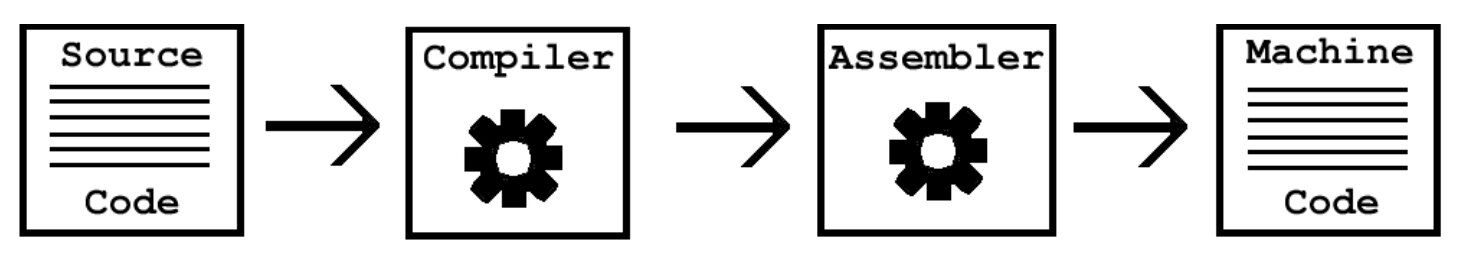
\includegraphics[width=.8\textwidth]{media/Source2Executable.jpg}
    \caption{Quellcode (engl. ``source code'') wird in ausführbaren Maschinencode umgewandelt \cite{stallman2002}}
\end{figure}

Hier als Beispiel der Source Code zu einem simplen Programm \textit{helloworld.c} geschrieben in der Programmiersprache C, welches in der Konsole ein simples \say{Hello World} ausgibt:

\lstset{language=C}
\begin{lstlisting}
#include <stdio.h>

int main() {
    printf("Hello World\n");
    return 0;
}
\end{lstlisting}
Ein Teil der kompilierten, ausführbaren Version des Programmes \textit{./helloworld} sieht aber so aus:
\begin{lstlisting}
0011010001100000010111110110111101101100011001110110001001101111011011000110000101100100
1111101101111011101000111001101110010011000010101111100000000000000110100011100000111100
1101010110001100000000011011010110111101101100011100000111010001100101011001000110010100
0000010111001011111000000000000000000000011010010000000011001000101111101011111011011110
1100011001110110001001101111011011000110000101100100010111110110111101110100011100110111
0000000000000001101001001000001100001010111110111100001110101011001100101111101101110011
\end{lstlisting}

Wie zu sehen ist, geht bei diesem Prozess des Kompilierens die Lesbarkeit für den Menschen grösstenteils verloren. Um ein Programm ausführen zu können, braucht der Nutzer also keinen Zugang zum Quellcode. Doch wenn er wissen will, was das Programm macht - es könnte ihn ausspionieren oder andere bösartige Dinge im Hintergrund machen - oder einfach das Programm verändern will, braucht er unbedingt Zugang zum Source Code.\\

\newpage

\subsubsection{Lizensierung}
% ENG: The differences of different source code models and their licenses have been already discussed in this paper (?). The reason the GNU General Public License Version 3 (short: GPL v3) was chosen because it is one of the most popular and strongest copyleft licenses that suits the application.
Grundsätzlich gibt es die  Unterscheidung zwischen freien Softwarelizenzen und proprietären Softwarelizenzen. Doch auch bei Open Source Software gibt es verschiedene Lizenzmodelle, welche gewählt werden können. Diese lassen sich ziemlich gut in zwei Kategorien unterteilen: in \gls{permissive} und in \gls{copyleft}.\\

Die Autoren dieser App halten Copyleft Software in ethischer und praktischer Hinsicht für die beste Wahl bei der Softwarelizensierung. Weshalb entschieden wurde, für dieses Softwareprojekt die \textit{GNU General Public License (GPL) Version 3} \cite{GPLv3} der \gls{fsf} zu verwenden, da diese eine der bekanntesten, strengsten und somit effektivsten Copyleft-Lizenzen ist.

\subsubsection{Philosophie (suckless)}

\begin{nicequote}{Many (open source) hackers are proud if they achieve large amounts of code, because they believe the more lines of code they've written, the more progress they have made. The more progress they have made, the more skilled they are. This is simply a delusion.}{https://suckless.org Manifest \cite{suckless}}
\end{nicequote}

% ENG: (Nowadays) a lot of Open Source Developers pride themselves in writing software with much features that cater to the non-technical enduser. This results in having a large codebase, which gets bigger and bigger with every release. This makes it harder to maintaining the ever growing codebase, more and more bugs occurs, security and (most importantly) performance struggles under these conditions. This degrades the quality of software technology as it is the mainstream narrative to ``save time and money''.\\

Eine grosse Anzahl Open-Source-Entwickler sind stolz darauf, Software mit scheinbar möglichst vielen Features zu schreiben. Dies führt zu einer grossen Codebasis, die mit jedem Release grösser und grösser wird. Dadurch wird es schwieriger, die ständig wachsende Codebasis zu unterhalten. Es treten immer mehr Fehler auf, die Sicherheit und - vor allem - die Leistung leidet unter diesen Bedingungen. Dies führt zu einer Verschlechterung der Code-Qualität der Software, da es die gängige Praxis ist, ``Zeit und Geld zu sparen''. \cite{bhattacharya2020}\


% ENG: This is where the \textit{suckless philosophy} comes in place: It aims at making software with simplicity in mind: Less source lines of code to not render the project unmaintainable in similar way as mentioned above. This way of programming is a lot more difficult, but the struggle is most of the time worth it. This coding philosophy also incentives (quality) code rewrites - which happens a lot less with bloated software counterparts - that gives the user more alternatives to choose from.

Hier kommt nun die \textit{Suckless Philosphie} ins Spiel: Sie zielt darauf ab, Software mit Hinblick auf Einfachheit zu entwickeln: Weniger Quellcodezeilen, um das Projekt nicht in ähnlicher Weise unüberschaubar zu machen, wie oben erwähnt. Diese Art zu programmieren ist viel schwieriger, aber der Aufwand ist es meistens wert. Diese Programmierphilosophie bietet auch Anreize für das qualitativ hochwertige Neuschreiben von Programmen, was bei der sogenannten \textit{Bloated Software \cite{bhattacharya2020}} viel seltener vorkommt, dazu gibt es dem Benutzer mehr Alternativen zur Auswahl.


\paragraph{Hintergründe, Technologisch, UNIX, KISS}
Die \textit{Suckless Philosophie} ist aber längst nicht die erste Philosophie im Softwarebereich, welche auf Simplizität beruht; so beispielsweise eine beliebte Definition der altbekannten \textit{UNIX Philosophy}:

\begin{nicequote}{This is the Unix philosophy. Write programs that do one thing and do it well. Write programs to work together. Write programs that handle text streams, because that is a universal interface.}{A Quarter Century Of UNIX \cite{salus1994}}
\end{nicequote}

Bekannt ist auch das \textit{KISS Prinzip}: \say{Keep it simple, stupid}. Dieses Prinzip kommt ursprünglich vom U.S. Admiral Stroop, der das \say{Project KISS} 1960 ins Leben gerufen hatte, welches die Verlässlichkeit verbessern und die Kosten für amerikanische Militärausrüstungen senken soll. \cite{dalzell2009} Gerne wird dieses Prinzip zitiert, wenn jemand der Meinung ist, unnötige Komplexität sei vorhanden in einem Softwareprojekt.


\subsection{Arbeitsziele}

Wir wissen, was ein Email Client können muss, und haben nicht vor, eine App zu designen, welche vollkommen überladen ist mit Funktionen die keiner braucht.\\

Die App soll die Basisfunktionen eines klassischen Email Clients erfüllen. Dazu gehören das Lesen, Schreiben, Empfangen und Versenden von Emails, 
das Öffnen und Anfügen von Anlagen, die Setzung einer Email-Signatur und das Erstellen und Speichern von Entwürfen. 
Ebenso soll er verschiedene Ordner unterstützen, wie z.B. einen Spam/Junk oder einen Archiv Ordner. 
Dazu soll es möglich sein E-Mails visuell sortieren zu können, beispielsweise indem die Ordner im Client nach Datum des Empfangs oder dem Absender sortiert werden können. E-Mails sollen markiert, gelöscht und weitergeleitet werden können und es soll eine Suchfunktion für jeden Mailordner geben. \\

Ebenso soll es einen Account Manager geben, was voraus setzt, dass es möglich ist, sich mit verschiedenen 
Accounts anzumelden und diese bei Bedarf zu wechseln. Beim Anmelden einer E-Mail, soll es dem Nutzer leicht gemacht werden, mit eingebauten Konfigurationen für beliebte 
Emailprovider in der Schweiz. Darunter diese Anbieter: stud.edubs.ch, gmail.com, gmx.ch, outlook.com, yahoo.com, icloud.com, hotmail.com, web.de. \\


Ein Element, welches fast jede App heutzutage besitzt, sind Pushnachrichten, welche auch eingebaut werden sollen. Dabei sollen neue Nachrichten mit dem Absender und dem Beginn der E-Mail angezeigt werden. 
Dies soll ein weiteres Feature der App sein. Wie es für leichte Email-Clients oft üblich ist, werden Bilder erst angezeigt, sobald es der Nutzer ausdrücklich möchte. Dieses Verhalten soll in den App-Einstellungen steuerbar gemacht werden. Eine sehr praktische Funktion soll sein, dass E-Mail-Adressen gespeichert werden und beim Schreiben einer neuen E-Mail direkt verfügbar sind und ausgewählt werden können. %Ob diese Funktion sinnvoll ist, ist fraglich, da viele Leute keine Emailaddressen auf der Kontaktapp ihres Handys speichern.
\\

Das letzte Feature soll sein, dass Links direkt in einem Browser geöffnet werden können. Die Einstellungen sollen zudem das Farblayout der App, die Synchronisationsintervalle und Einstellungen an den Pushnachrichten ändern können, Kontaktlisten verwalten und Einstellungen zur Privatsphäre beinhalten.


Im Unterschied zur Konkurrenz soll diese App so programmiert werden, dass sie alle nötigen Grundfunktionen für einen Email Client auf dem Smartphone beinhaltet, aber schneller starten soll als die Apps der Konkurrenz, weniger Speicherplatz und Ressourcen verbrauchen und nicht mit unnötigen Funktionen überladen sein soll.\\


Ein Pluginmanager soll auch eingebaut werden, um weitere Funktionen, welche das Programm verlangsamen würden oder nicht für jedermann geeignet sind, hinzufügen zu können. Es existiert natürlich auch die Möglichkeit, nach Abschluss dieser Arbeit die App zu verbessern und auf Nutzerwünsche anzupassen, doch hier wurden jetzt die ungefähren, geplanten Grundfunktionen genannt, um die Ziele der Funktionalität besser zu beleuchten.\\
Es wurden viele Ziele gesetzt und es wurde angenommen, dass noch mehr erreicht werden kann. Weshalb dies nicht der Fall ist, wird noch genauer betrachtet.

\newpage

\section{Arbeitsprozess}

\subsection{Programmiermittel}

Um ein Programm, mit grösserem Umfang zu entwickeln, ist es nützlich, Hilfsmittel zu verwenden, welche sich grössere Projekte spezialisiert haben. 
Eines dieser Hilfsmittel sind \gls{vcs}. Diese sind eine sehr praktische Methode um Funktionen in ein Programm einzubauen ohne das Risiko,
das Programm komplett Überarbeiten zu müssen, wenn eine einzige Funktion einen Fehler hervorruft. In diesem Fall wurde \Gls{git} als VCS genutzt, um für jegliche Funktionen
einen eigenen \Gls{branch} zu erstellen und diesen wieder mit dem Hauptbranch zu \glspl{merge}, wenn die Funktion fertig ist.\cite{git} \cite{github} \\

\begin{figure}[H]
    \centering
    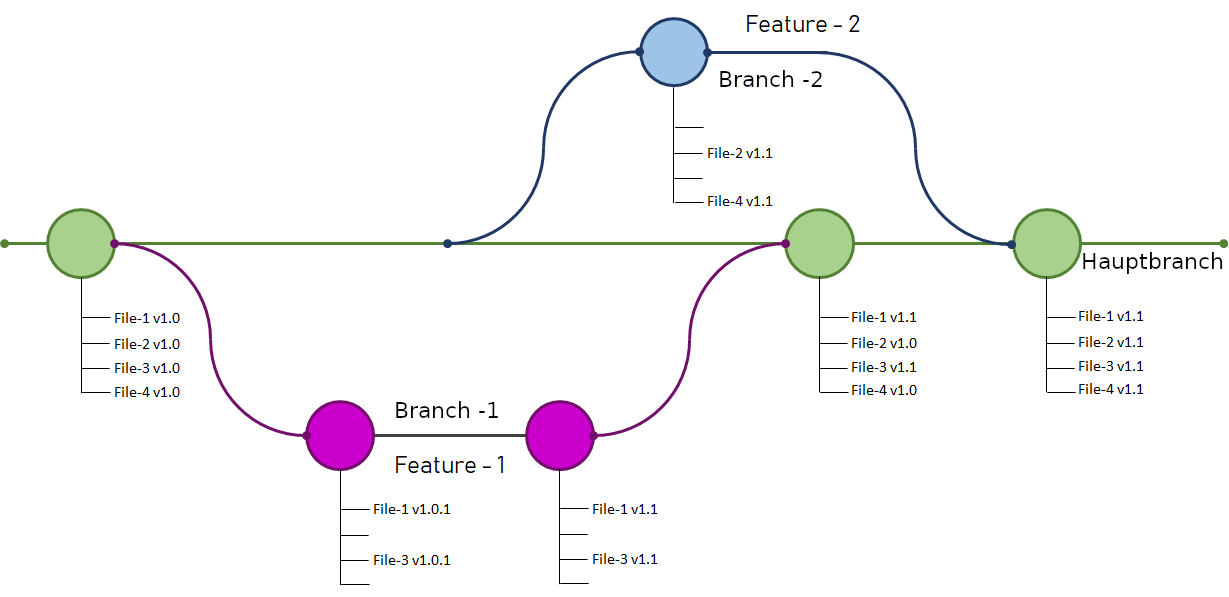
\includegraphics[width=.8\textwidth]{media/gitflow2.png}
    \caption{parallele Featureentwicklung mit Git \cite{gitflowBlog}}
\end{figure}

Um zu zweit an einem Projekt gleichzeitig zu arbeiten, gibt es viel Möglichkeiten, sich das aktualisierte Projekt zur Verfügung zu stellen. Die \say{Einfachste} ist, sich das 
Projekt immer wieder zu mailen, wobei schon nur bei Textarbeiten dabei Probleme auftauchen können, weshalb bei diesem Projekt \Gls{github} 
verwendet wurde. Über GitHub konnten die einzelnen Versionen des Programms, welche durch den Gebrauch von \gls{git} entstanden sind, geteilt werden. 
Auf GitHub ist das Programm öffentlich und wird dadurch auch quelloffen. Es kann aber nicht durch eine dritte Person ohne Einwilligung von Noah in den Source-Code
des Programms geschrieben werden. Falls dies aber der Fall gewesen wäre, würde die dritte Person als mitwirkende Person auf GitHub aufgelistet werden. \cite{github} \\

Beim Programmieren einer Arbeit dieser Grösse, erweist es sich besonders nützlich, ein \glspl{ide} zu verwenden. Es ist zu \gls{android-studio} gegriffen worden, weil sich dieses 
IDE speziell auf die Android Entwicklung spezialisiert hat. \gls{android-studio} besitzt viele Hilfsmittel, welche das Programmieren einer Androidapp erleichtern. Zum Beispiel ist der
"Visual Layout Editor"\ eine grosse Hilfe beim Designen. \gls{android-studio} bringt auch einen \gls{compiler} und einen \gls{emulator} mit sich, womit eine \textit{debug} \gls{apk} und eine
\textit{release} \gls{apk} version der App erstellt werden kann. Um die App zu testen, wurde öfters ein \textit{debug} APK File erstellt und auf einem \gls{emulator} aus \gls{android-studio}
getestet. Mit \gls{android-studio} können auch Apps mit speziellen Keys unterzeichnet werden, damit sie im Google Play Store veröffentlicht werden können.
Die App sollte aber nicht nur auf Emulatoren laufen, um auch das Gefühl des Designs besser zu empfinden oder den Gebrauch im Alltag zu testen, wurde die \gls{adb} benutzt.
Mit \gls{android-studio} können auch Daten über die Effizienz der App aufgenommen werden. 
\cite{android-studio} \\

Open-Source Programme wurden bei dieser Arbeit mehrmals genutzt, um gewisse Funktionen einzubauen und ein Gefühl für das Programmieren solcher Funktionen zu bekommen. Die Programme
waren sehr 
hilfreich beim Lernen, da die Autoren teilweise noch gar keine Erfahrung in gewissen Bereichen hatten. Was genau aus diesen Programmen entnommen wurde und um welche Programme es sich handelt, wird 
genauer im Anhang besprochen. 



\subsection{Programmstruktur}

\subsubsection{Hauptziele}
Gemäss den Zielen soll die App eine Verbindung mit einem Server erstellen und mit ihm interagieren können. Das heisst, sie soll die Informationen über einen Account, die der 
Nutzer eingibt, überprüfen können und weiter die Emails, die ein Nutzer auf einem \gls{server} hat, herunterladen. Ebenso soll die App Nachrichten weiter über einen Server verschicken können. 
Um das zu realisieren, haben sich die Autoren nach passenden \glspl{library} für Java umgeschaut. Das Resultat dieser Suche waren zwei Libraries. \\



Weil nach dem Herunterladen der Nachrichten vom Server viele Daten gespeichert werden müssen, muss eine Möglichkeit her, wie diese Daten möglichst schnell, 
und der Einfachheit halber mit einer gewissen Abstraktion, in einer sinnvollen Datenstruktur gespeichert werden können. Dazu taugte eine \gls{database}. Um dies zu erreichen, 
las sich einer der Autoren in ein Buch ein. Dieses Buch sollte ihm Aufschluss über das Erstellen einer Database geben.  \\

Es wurde klar, dass eine Database für Android meist mit \gls{sql} oder \gls{sqlite} geschrieben wird. Jedoch sind diese Sprachen nicht wirklich handlich und es
liess sich auch nicht mit dem Zeitplan verknüpfen eine weitere Programmiersprache zu lernen, weshalb zu Room gegriffen wurde. Room ist eine abstrakte Klasse über SQLite 
und kann mit dieser kommunizieren. Mit ihr können SQL \glspl{query} fast vollständig in Java geschrieben und ausgeführt werden. Ebenso ist Room für die Fehlersuche besser geeignet, 
weil es beim compilen der App die SQL queries und \glspl{entity} überprüft. \cite{roomInfo} \\

\newpage

\begingroup
\setlength{\intextsep}{7pt}
\setlength{\columnsep}{15pt}

\begin{wrapfigure}{r}{6cm}
\centering
    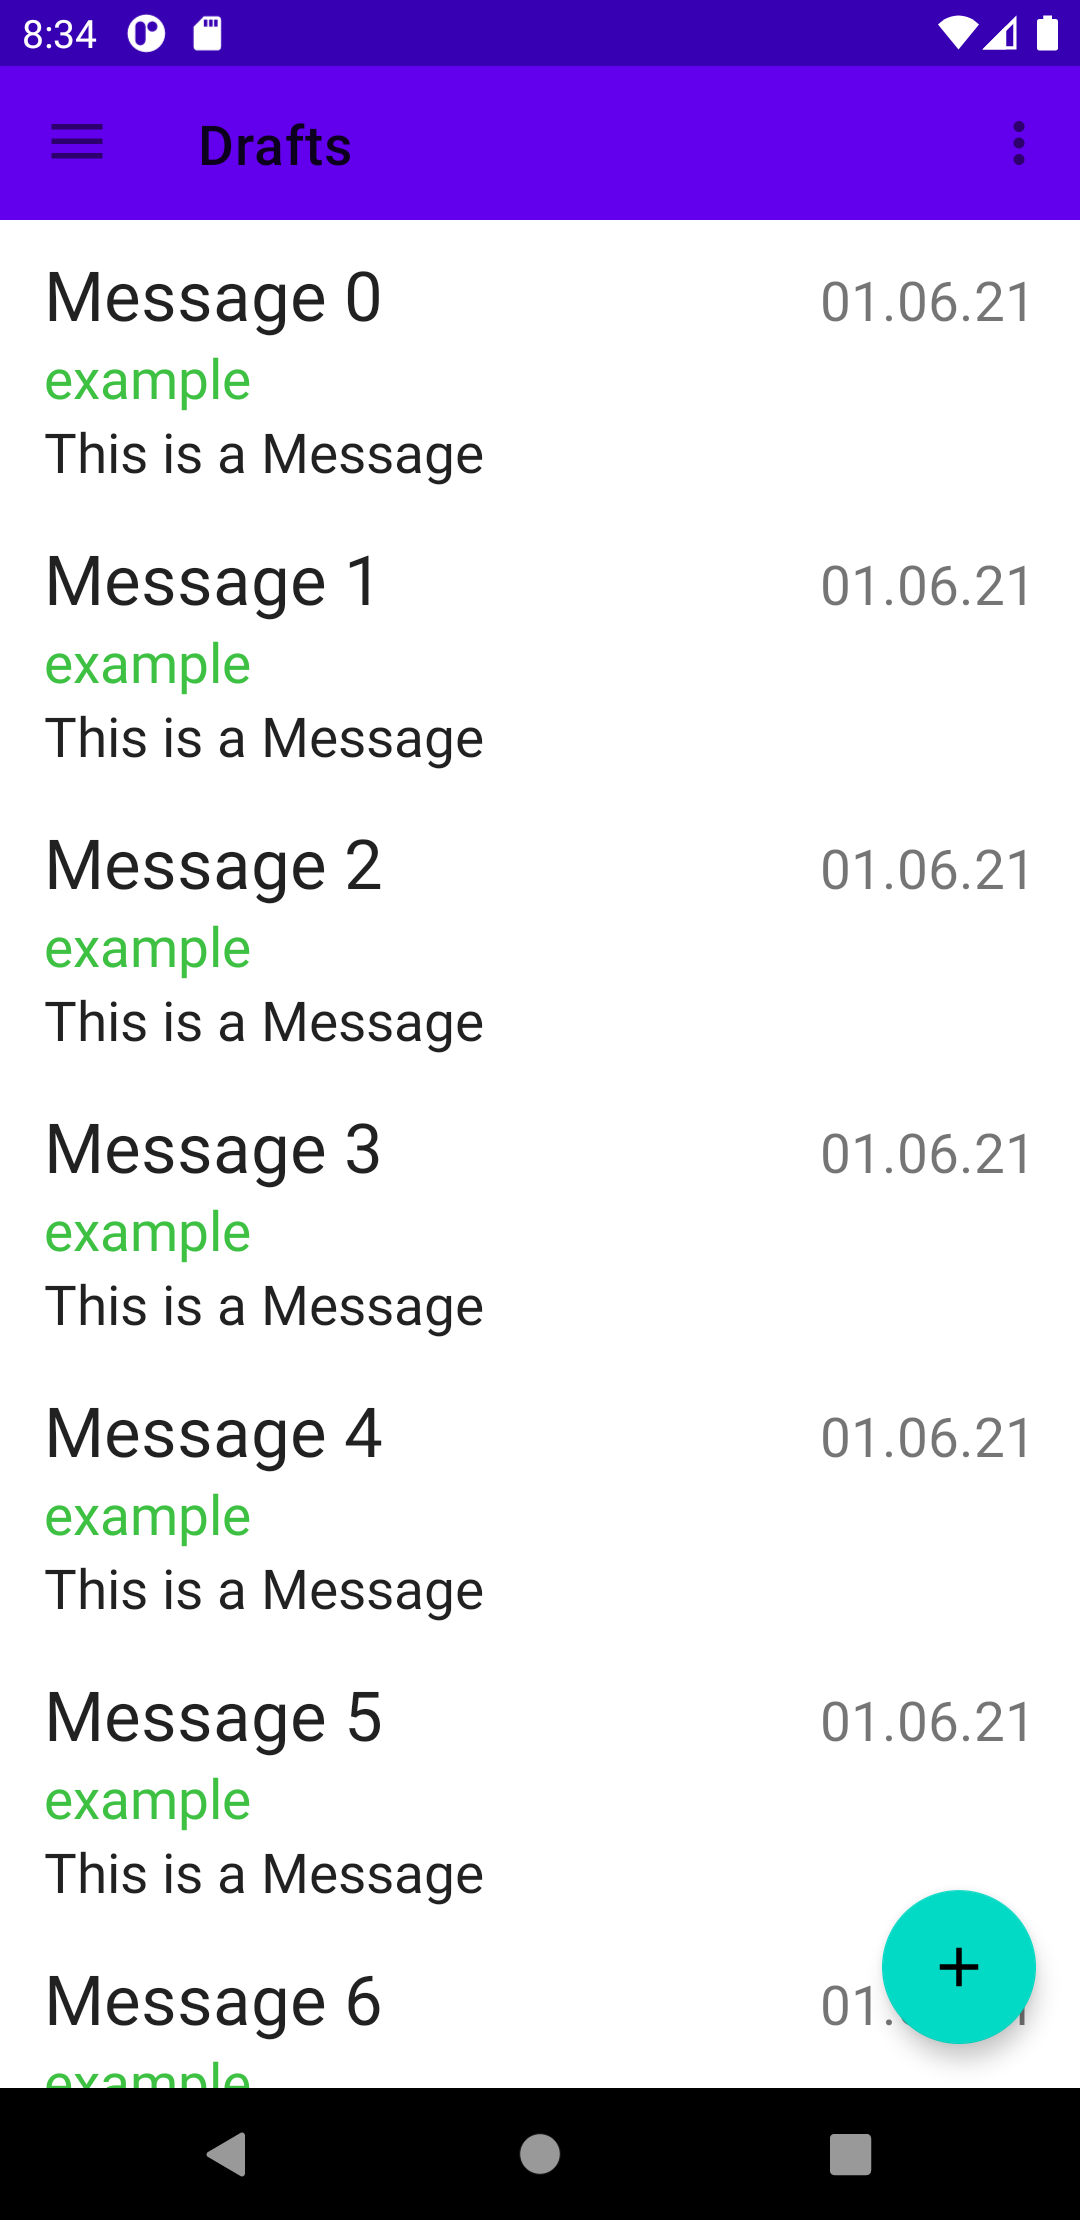
\includegraphics[scale=.12]{media/RecyclerViewScreenshot.png}
\caption{Beispiel vom RecyclerView}
\end{wrapfigure}

\nohyphenation

Damit die heruntergeladenen und gespeicherten Nachrichten auch angezeigt werden können, benötigt es ein Interface. Dieses sollte so schlicht und ordentlich wie möglich gehalten werden. 
Die \gls{recyclerview} Library ist eine optimale Möglichkeit, Daten in Form von Nachrichten als eine Auflistung zu zeigen. Sie bringt einen Vorteil gegenüber einer \glspl{list} mit und zwar
verwendet sie \glspl{view} wieder, die angezeigt wurden. Was dem Recyclerviewer einen Vorteil im Punkt Effizienz gegenüber der Liste bringt. \cite{recyclerViewRecycle}

Neben der Recyclerview Library werden auch andere Bibliotheken gebraucht, um das \gls{user interface} zu erstellen. Einer dieser libraries ist Material oder Material Design. 
Den Autoren hat sie schlicht gefallen und sie ist nicht schwer zu benutzen, weshalb diese Library genutzt wurde. Sie ist nach ganz klaren Prinzipien aufgebaut 
und von Google erstellt worden, um hochwertige Designs zu kreieren. \cite{materialDesigne}

\endgroup

\subsubsection{Aufbau}

Die App kann grob in drei Teile unterteil werden. In \textit{User Interface}, in \textit{Database} und in \textit{Serververbindung}. 

\begingroup
\setlength{\intextsep}{7pt}
\setlength{\columnsep}{15pt}

\begin{wrapfigure}{r}{10cm}
\centering
    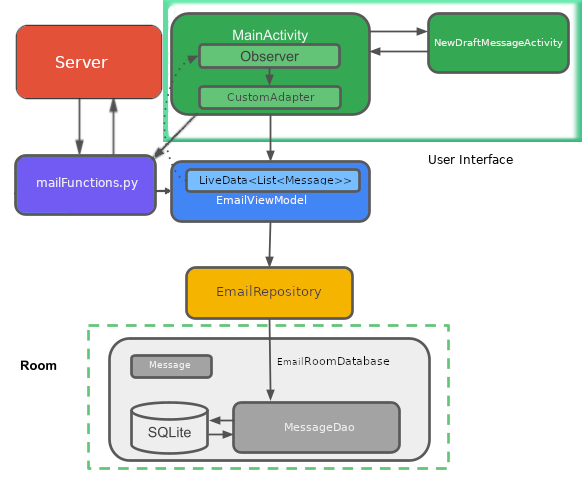
\includegraphics[scale=.52]{media/AppStructureFull.png}
\caption{grober Aufbau der App}
\end{wrapfigure}

\nohyphenation

Diese drei Komponenten bilden zusam-men die App, wobei der Teil der Serververbindung nicht immer aktiv ist. Er wird von dem User Interface
aufgerufen, wenn sich zum Beispiel ein neuer Nutzer mit einem Emailaccount anmelden möchte. Dann werden die Accountdaten an den Server geschickt und überprüft.
Wenn diese korrekt sind, werden alle Nachrichten, die dieser Nutzer auf dem Server hat, heruntergela-den und weiter an die Database gegeben. Abgesehen von dem 
Speichern der Nachrichten, die frisch vom Server kommen, macht die Database nur noch zwei Dinge. Sie kann durch das Interface entstandene Nachrichten so abspeichern, dass sie 
vom \textit{User Interface} im Ordner \textit{Draft} angezeigt werden. Und die \textit{Database} kann weiter gespeicherte Nachrichten so bearbeiten, dass sie vom 
\textit{User Interface} in einem anderen Ordner angezeigt werden.

\endgroup

\subsubsection{Startup UI}


%I then made the app more functional, so that you have a base GUI with a drawer, a menu in the bottom and in the drawer navigation menu you can tap on the «Add Email» Button and a popup window will come up asking you for name, email and password. Even the save and cancel button work. Now we only need a functionality to save this information to a string somewhere in the main activity.\\

\begin{figure}[H]
\centering
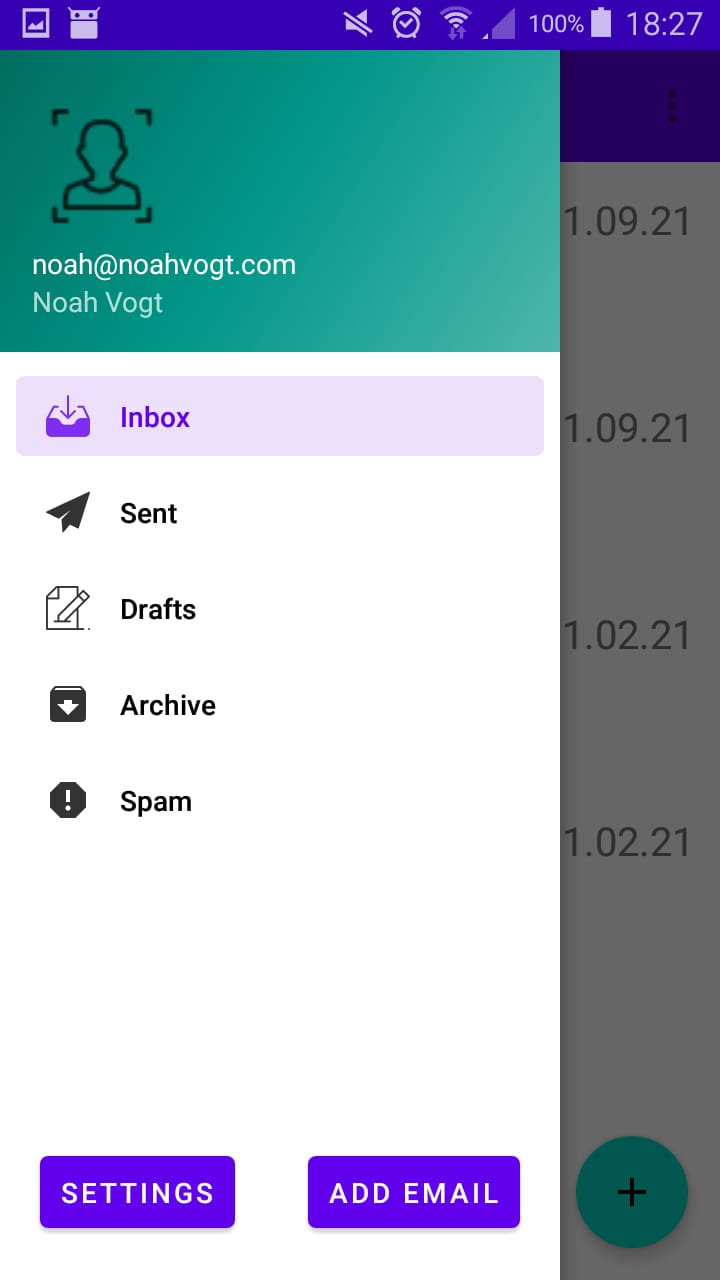
\includegraphics[width=.32\textwidth]{media/drawer.jpeg}
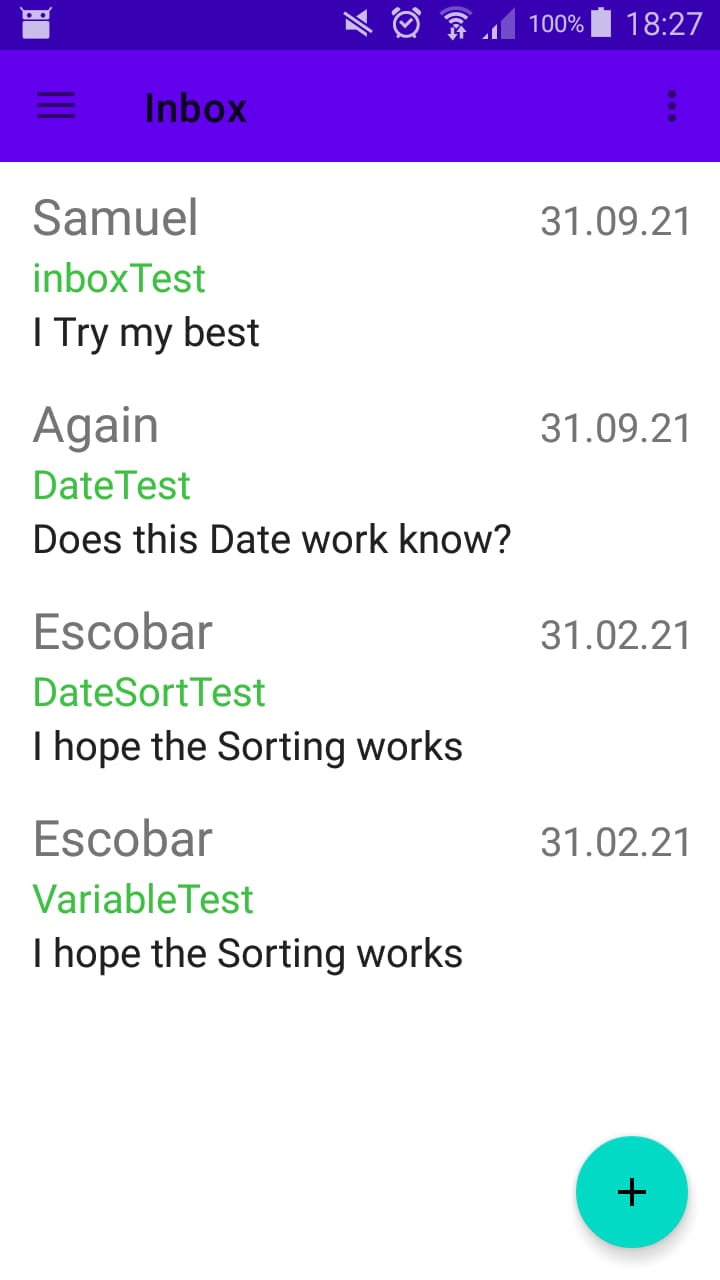
\includegraphics[width=.32\textwidth]{media/inbox.jpeg}
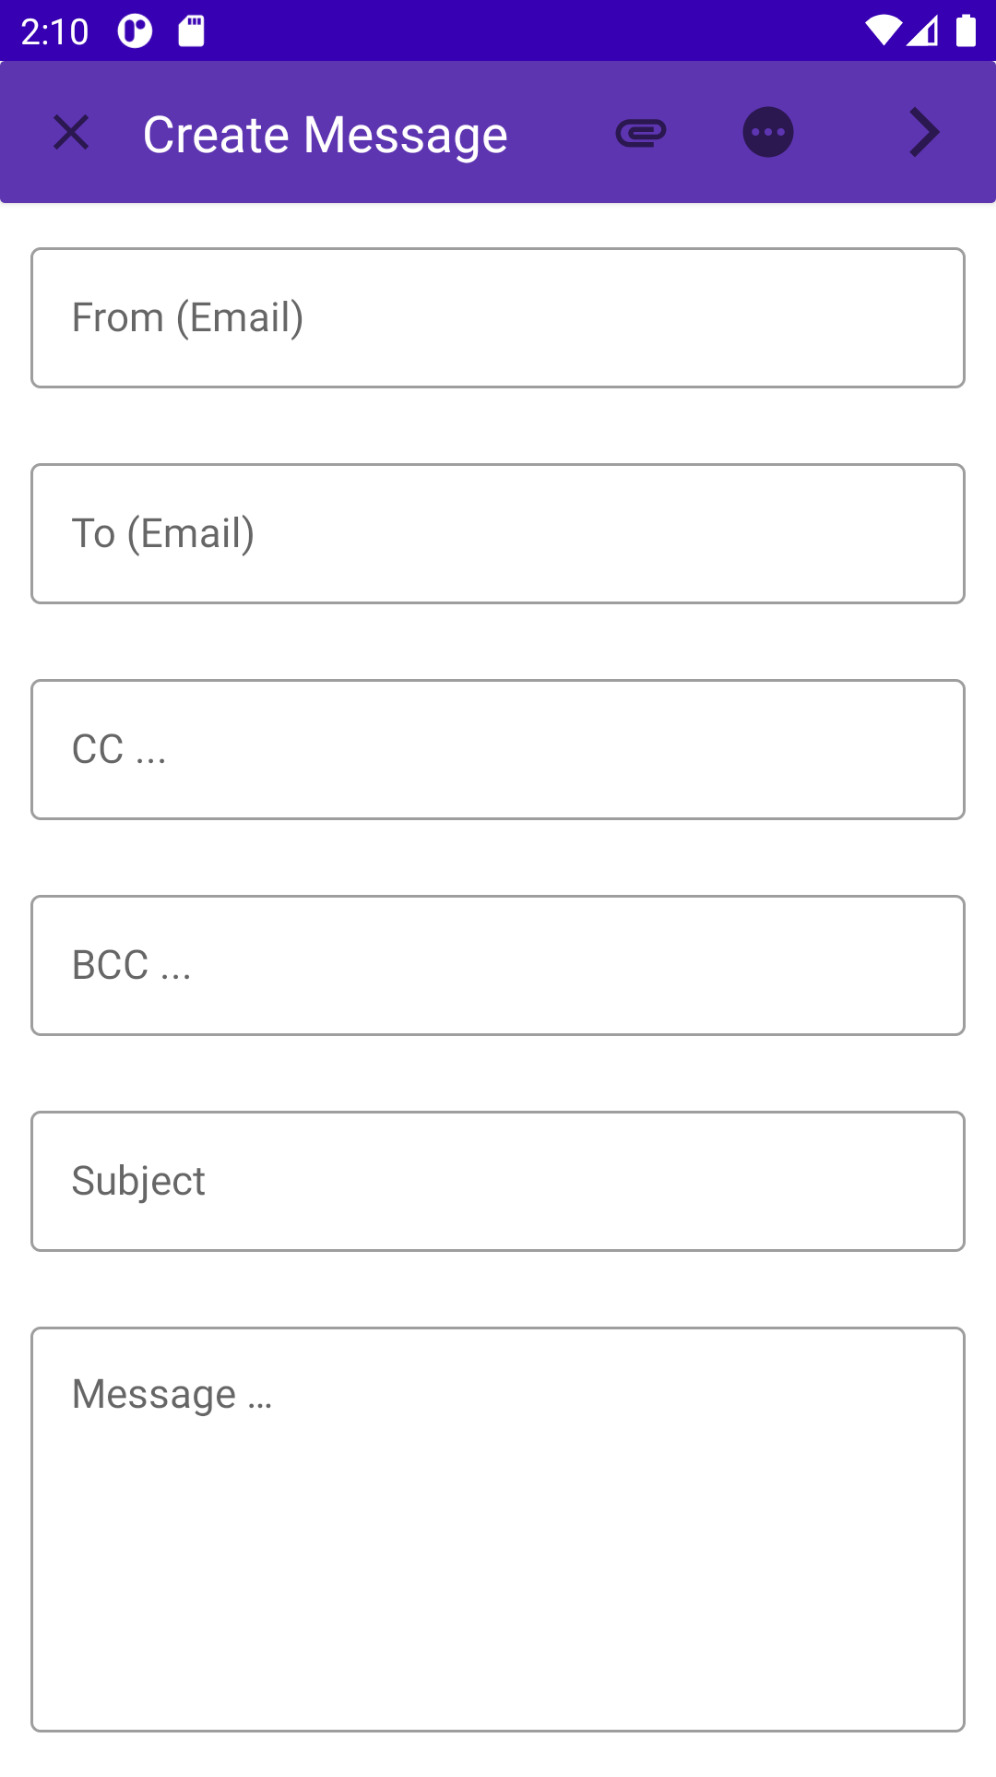
\includegraphics[width=.32\textwidth]{media/emailWriter.png}
\caption{die Startup UI von snailmail}

\end{figure}

Wenn man die App startet, sieht man als allererstes die durchscrollbare Inbox (siehe mittleres Bild), hier mit vollkommen arbiträren Testdaten. Bei den 3 Menüpunkten soll im weiteren Verlauf der Entwicklung die Funktionalität hinzugefügt werden, Emails zu sortieren und zu durchsuchen.\\

Wenn im Bild in der Mitte unten rechts das Pluszeichen angetippt wird, erscheint ein Fenster, wo man eine neue Email schreiben kann (Bild rechts). Man kann sie entweder versenden, oder als Entwurf speichern. Wenn der Nutzer sich mit einem Account angemeldet hat, wird die Adresse des Absenders - im Bild entspricht das dem Textfeld mit dem Platzhalter \say{From (Email)} - automatisch mit der aktuellen Email Adresse vervollständigt.\\

Wenn man im mittleren Bild oben links auf das sogenannte \say{Hamburgermenü} drückt, oder wie auf vielen anderen Apps auch von links nach rechts swiped (dt. streicht), erscheint der sog. \say{Drawer} (im Bild links ersichtlich). Dort sieht man den eingeloggten Account, die verschiedenen Mailboxen und ein paar Buttons, um zu den Einstellungen zu gelangen (unten links), einen neuen Email Account hinzuzufügen (unten Mitte) und um zum Account Manager zu gelangen (durchs Tippen auf das Profilbild). Dort kann auf eine andere Mailbox geklickt werden, sodass diese ausgewählt und geöffnet wird.


\newpage

\subsubsection{Account Management}

Wenn man im Drawer den \textit{Add Email Button} drückt, erscheint ein Pop-up Fenster, in dem man seine Anmeldedaten für ein neues Email Konto angeben kann. Da ein Mailserver aber auch von gewissen Standardeinstellungen, wie beispielsweise vom standardmässigen IMAP Port 993 (wie definiert von der \gls{ietf} in der IMAP Spezifikation rfc9051 \cite{rfc9051}) abweichen kann, werden in diesem Fenster zuerst die Standardeinstellungen getestet, indem eine kurze Anfrage an den Server ausgeführt wird. Zuerst wird geschaut, dass nicht bereits ein Account mit der gleichen Email Adresse wie der zu Hinzufügende, wobei dann eine Meldung erscheint für den Nutzer. Dann werden die Anmeldedaten anschliessend mit der Funktion \textit{checkConnection} überprüft, um zu überprüfen, ob man sich mit diesen zum Mailserver verbinden kann.\\

\lstset{language=python}
\begin{lstlisting}
def checkConnection(host, username, password, port):
    try:
        connection = imaplib.IMAP4_SSL(host, port)
        connection.login(username, password)
        connection.logout()
        return True
    except Exception as e:
        print("host: " + host)
        print("username: " + username)
        print("port: " + str(port))
        print(str(e))
        return False

\end{lstlisting}

Wenn die Anfrage erfolgreich ist, werden die Anmeldedaten in der App gespeichert. Wenn nicht, erscheint ein neues Dialogfenster, in welchem der Nutzer gefragt wird, ob er noch weitere Angaben angeben möchte, um diese dann testen zu können.\\

Wie schon in Punkt 3.2.3 erwähnt, muss man im \textit{Drawer} auf das Profil klicken, um zum Account Manager zu gelangen, wo dann ein Dialogfenster erscheint. Zuerst wird der Benutzer vom Programm angewiesen mit der Nachricht \say{select Account} ein Konto im Drop-Down Menü auszuwählen. Dann kann er eine Aktion ausführen, indem er einen der korrespondierenden Knöpfe drückt, oder mit \say{exit}-Button das Dialogfenster wieder schliessen.\\

\begin{figure}[H]
\centering
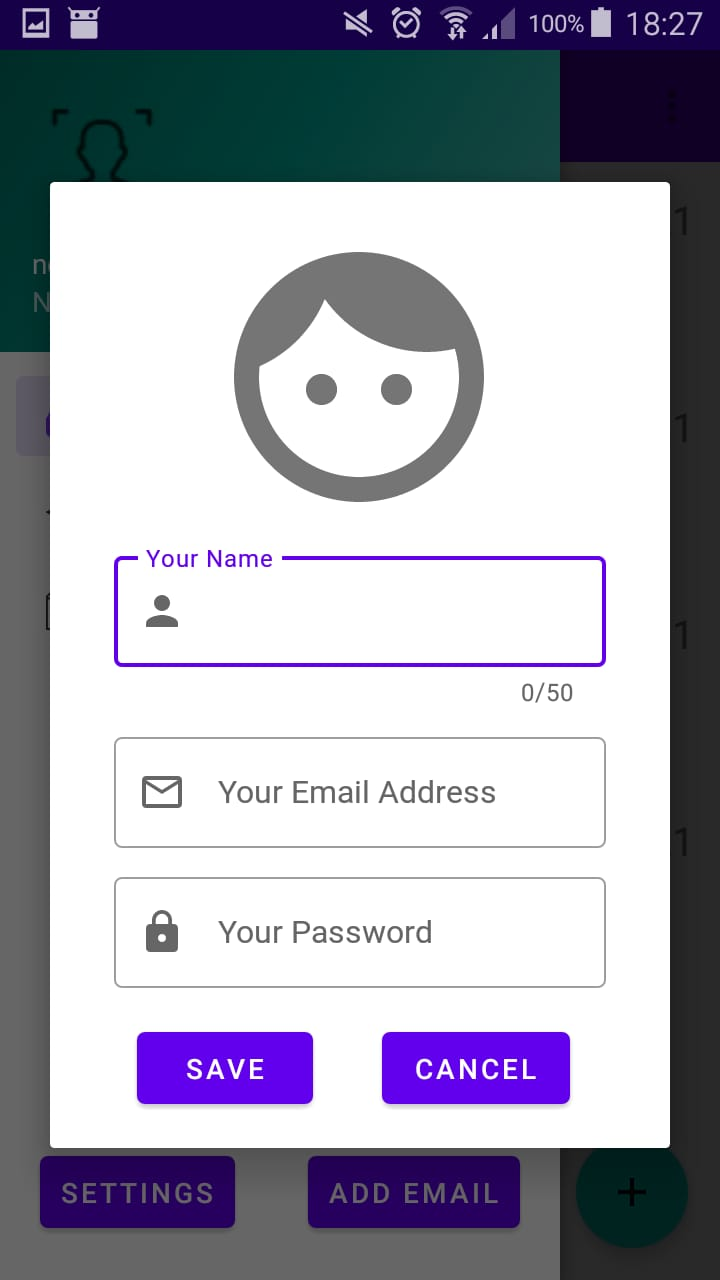
\includegraphics[width=.32\textwidth]{media/plain-add-email.jpeg}
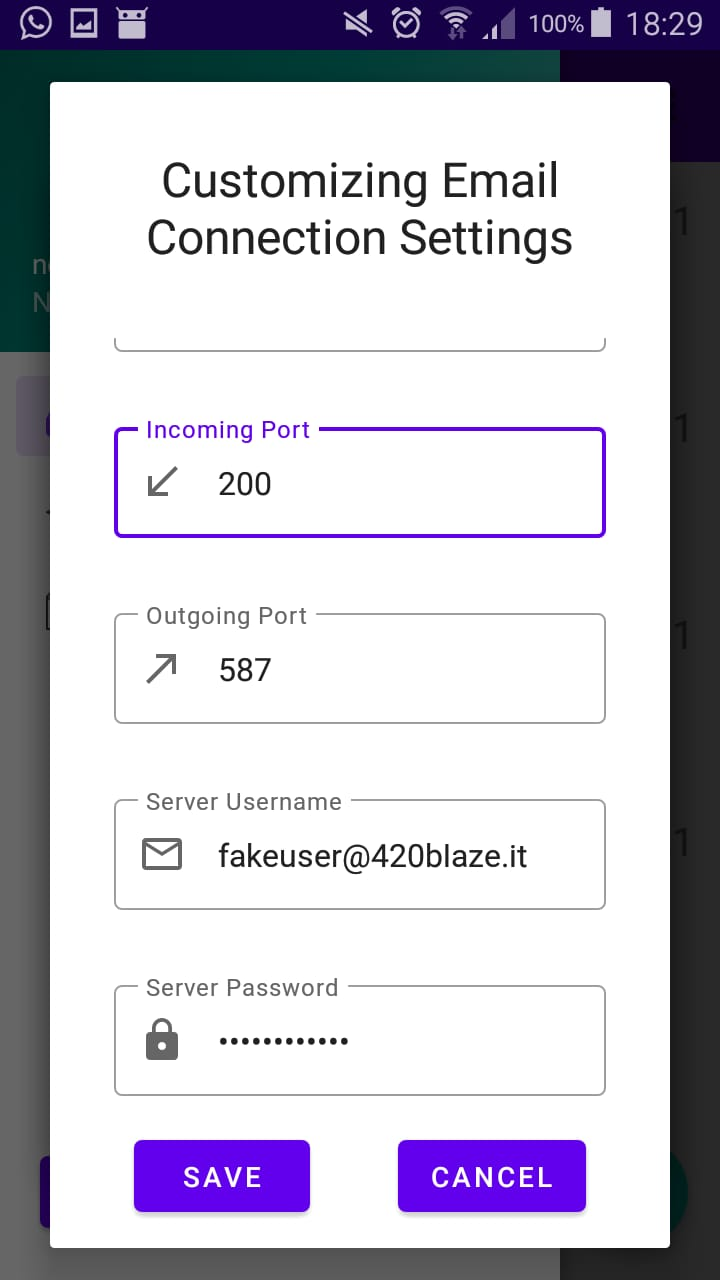
\includegraphics[width=.32\textwidth]{media/advanced-add-email.jpeg}
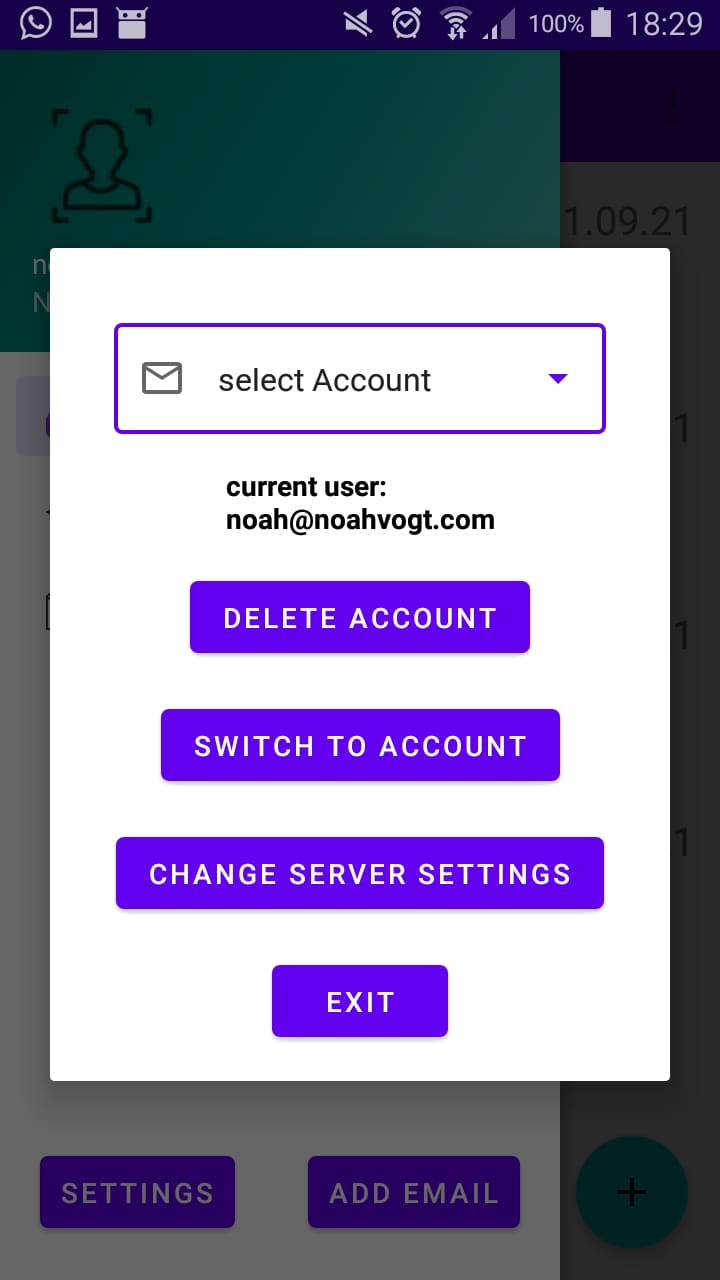
\includegraphics[width=.32\textwidth]{media/plain-account-manager.jpeg}
\caption{das Account Management}

\end{figure}

Der Nutzer kann entweder den ausgewählten Account löschen, zu ihm wechseln, oder seine Server Settings ändern. Beim Letzteren erscheint das gleiche Menü wie in den erweiterten Einstellungen, um einen neuen Account hinzuzufügen. Wenn der Nutzer seine neuen Mailservereinstellungen speichern will, wird zuerst geschaut, ob die App sich immer noch mit dem Mailserver verbinden kann. Wenn nicht, erscheint eine Fehlermeldung für den Nutzer und die neuen Angaben werden \textit{nicht} gespeichert.\\

Zur Hilfe wird im Dialog des Account Managers die ganze Zeit zur Hilfe der aktuell aktive Account angezeigt. Nach jeder der Account Manager Aktionen werden immer noch diese Anzeige und die Textfelder im Drawer, wo der Nutzer seinen zur Zeit aktiven Email Account sehen kann, in Echtzeit aktualisiert.


\subsubsection{Recyclerviewer}
Wie im Kapitel \say{Hauptziele} schon angedeutet, braucht es einen Recyclerviewer um Nachrichten aufgelistet anzuzeigen.
Ein Recyclerviewer ist in fünf grundlegende Teile aufgeteilt. 

\begin{enumerate}

    \item Das Recyclerview Objekt, welches ein Container ist und in das User Interface eingebaut wird. 
Es beinhaltet verschiedene Views, welche nochmals unterteilt werden können. In einer View wird in diesem 
Fall eine Nachricht eingebaut mit dem Absender, der Absendezeit, einem Betreff und dem Endsender der Nachricht. 

\end{enumerate}

\begin{enumerate}

    \setcounter{enumi}{1}
    \item Der Layoutmanager. Er ist für die Form einer einzelnen View verantwortlich. 
Der Layout manager kann auch wieder in drei Arten unterteilt werden. Der Linearlayoutmanager sorgt für eine 
Horizontale oder vertikale Unterteilung einer View. Hingegen führt der Gridlayoutmanager zu einer horizontalen 
und vertikalen Unterteilung der View. Für den Email-Client bietet er die  
beste Oberfläche, um Nachrichten darzustellen. Es gibt nämlich noch den den Staggeredgridlayoutmanager, welcher 
für eine versetzte Unterteilung der View sorgen kann. Dies ist aber für einen Email-Client unbrauchbar. 

\begin{figure}[H]
    \centering
    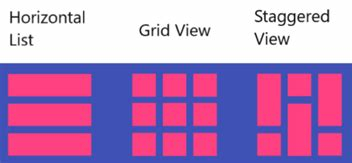
\includegraphics[width=.4\textwidth]{media/RecyclerviewLayoutManagerCropt.jpeg}
    \caption{Layout Manager Recyclerview \cite{LayoutManagerPicture}}
\end{figure}

    \item Der View Holder beschreibt die Position einer View oder Metadaten innerhalb des Recyclerviewers.

    \item Der Adapter ist wohl eines der wichtigsten Teile des Recyclerviewers. Er sorgt für das Erstellen des ViewHolder-Objekts und
bindet auch die Daten aus der Database an den View Holder

    \item Die Database ist das Herzstück dieser App und wird auch für den Recyclerviewer verwendet, um die 
        Views mit den richtigen Informationen zu füllen. \cite{RecViewQue} \cite{RecViewQue2}

\end{enumerate}

Die Wahl des Layoutmanagers wurde sehr schnell getroffen. Es war klar, dass eine Nachricht nicht nur eine Information auf horizontaler Ebene anzeigen muss, sondern
z.B. auch das Datum nicht versetzt angezeigt werden soll. Deshalb wurde der Gridlayout Manager gewählt. \\

Mit Hilfe eines Open-Source Programms, welches eine Demonstration eines Recyclerviewers war, haben sich die Autoren über diesen informiert. \cite{RecViewApp}
Nachdem dieses Programm ausgetestet und beliebig modifiziert wurde, sollte es in die App eingebaut werden. 
Der erste Versuch scheiterte daran,
dass die App abstürzte, ohne einen Error zu melden. Nach einiger Zeit war die beste Lösung wieder an einen Punkt zu gehen, an welchem die App noch funktionierte, nur ohne vollständigen 
Recyclerviewer. Es dauerte einen ganzen Monat bis eine weitere Version mit Recyclerviewer bereit war. Nur diesmal funktionierte die App. \\

\subsubsection{Input Validation}

\begin{wrapfigure}{r}{5cm}
\centering
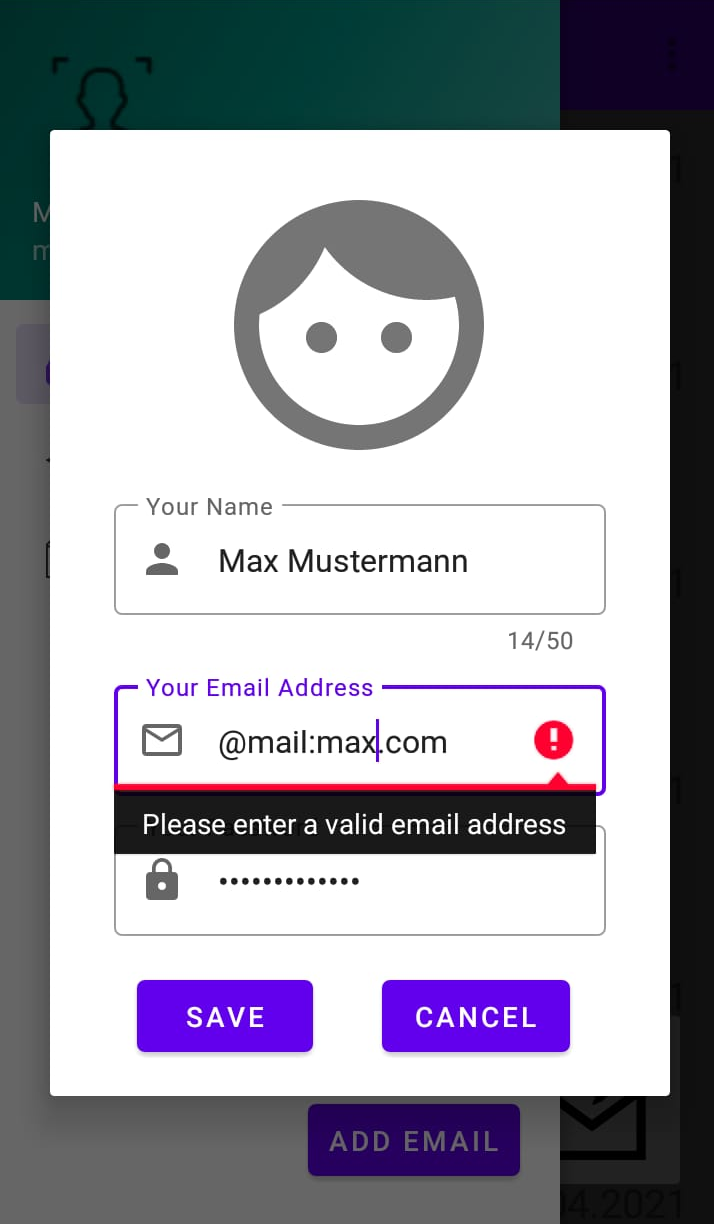
\includegraphics[width=.18\textwidth]{media/inputValidation.png}
\caption{Input Validation}
\end{wrapfigure}

Bei den meisten Textfeldern, wo der Benutzer etwas eingeben kann und es sinnvoll gecheckt werden kann gibt es in snailmail eine \textit{Input Validation}. Dort wird gecheckt, ob die Eingabe korrekt ist, also ob der Nutzer eine z.B. gültige Email Adresse eingegeben hat oder dass er ein Eingabefeld nicht leer lässt. Das Feld mit der falschen Eingabe wird rot markiert und der Nutzer weiss somit, an welcher Stelle er seine Eingabe korrigieren muss. Diese Praxis ist mittlerweile weitverbreitet und auf mobilen graphischen Oberflächen wurde diese von den Autoren als sinnvoll erachtet, weshalb sie auch in ihrer App davon Nutzen gemacht haben.

\subsubsection{Datenbank}

% Nachdem die Grundbausteine für den Recyclerviewer gelegt wurden, war es Zeit eine Database zu erstellen, welche die Informationen der Server 
% Speichern kann, da ein Ziel war POP3 anzubieten. Und mit IMAP muss die geöffnete Nachricht auch einmalig gespeichert werden. Dafür bietet sich eine Dabase gut an.
% \textbf{nicht sicher ob das Stimmt was ich hier schreibe}\\

Ein \textit{relational database management system} ist ein Datenbank-System, in welchem die Informationen als \textit{tables} gespeichert werden. 
Ein \textit{table} besteht aus Reihen und Spalten. Eine Reihe repräsentiert jeweils ein Object der Database und eine Spalte repräsentiert ein Wert eines Attributes. Im Fall dieser App
gibt es 9 Attribute und einen Objectkey. \cite{riccardi2001} \\


\begin{tabular}{ |p{1.6cm}  |p{1.1cm} |p{1.1cm} |p{1.05cm} |p{1.15cm} |p{1.15cm} |p{1.25cm} |p{1.75cm} |p{1.25cm} |p{1.15cm}|}
 \hline
 \multicolumn{10}{|c|}{Database Table} \\
 \hline
    ObejctKey &To & cc & bcc & from & date & subject & textContent & folder & seen  \\
 \hline
     01    &Valentin& null & null & Lennard & 01.03.13 & Schule &  Hallo Herr & Draft & true \\
 \hline
\end{tabular} \\

Der Objektkey wird dafür genutzt, das Objekt zu identifizieren und aufzurufen. Es können auch weitere Dinge mit dem Objektkey gemacht werden. 
Je nachdem, wie die Database eingelesen wird, kann am Objektkey festgestellt werden, zu welchem Zeitpunkt ein Objekt erstellt wurde. Bis auf seen und dem ObjektKey sind 
alle Attribute Strings. \\

\textit{To} ist das Attribut, welches angibt, an wen die Email geschickt werden soll, \textit{From} ist das genaue Gegenstück dazu. \textit{Cc} und \textit{bcc} sind die 
Email-Adressen, welche die Emails auch bekommen. Der einzige Unterschied ist, dass bei \textit{bcc} diese Adressen nicht einsehbar sind und somit nicht bekannte ist, wer diese Email auch liest. 

\textit{Date} gibt das Datum an, an welchem die Email verschickt wurde. \textit{Subject} ist ein Betreff für die Email und \textit{textContent} ist der Text, welcher in der Email verfasst wurde. 

Mit dem Attribut \textit{seen} war geplant, es von \textit{false} zu \textit{true} wechseln zu lassen, wenn der Nutzer eine ungelesene Nachricht öffnet. Dazu sollte dann die Schriftart,
in welcher die Nachricht im Recyclerviewer angezeigt wird, geändert werden. Leider hat diese Funktion es nicht in die App geschafft, aufgrund Zeitmangels und der eher 
geringen Wichtigkeit dieser Funktion. Dennoch wird sie sicher nach der Abgabe dieser Arbeit noch eingebaut. \\

Die Attribute \textit{To}, \textit{from}, \textit{date}, \textit{folder} und \textit{seen} wurden im Databaseconstructor als @NonNull definiert. Das heisst, sie müssen eingelesen werden und können 
nicht \textit{null} sein. Das macht soweit Sinn, weil eine Email bis auf \textit{seen} nicht ohne diese Angaben versendet werden können und ohne zu wissen, in welchem Ordner die Email einzuordnen ist,
kann die Email auch nicht richtig angezeigt werden. \\

Als Letztes gibt es noch das Attribut \textit{folder}, es gibt an, von welcher Art die Email ist. Es gibt in der App fünf Ordner. Sie heissen \textit{Draft}, \textit{Sent} 
\textit{Inbox}, \textit{Spam} und \textit{Archive}. Die Database kann nach einzelnen Attributen ausgelesen werden. So können die Emails mit den richtigen
folder Attributen in den richtigen Ordnern angezeigt werden. Jeder Ordner hat sein eigenes Fragment, welches aufgerufen wird, wenn der Ordner ausgewählt wird.
Wenn ein solches Fragment aufgerufen wird, wird auch die Database mit den richtigen Befehlen neu ausgelesen.  \\


%Für Android gibt es nicht viele Sprachen um eine Database zu erstellen. Die bekannteste ist SQLite .Jedoch ist SQLite nicht sehr simple und es kann sehr komplex werden, wenn
%die Database bis auf bytes genau Programmiert werden soll. Ebenfalls lag es nicht im Zeitplan eine weitere Programmiersprache zu lernen. Nach kurzer 
%recherche stellte sich heraus, dass es eine Library gibt, welche den Umgang mit SQLite vereinfacht und diese sogar mehr Sicherheit bietet.\\


\newpage
\begingroup
\setlength{\intextsep}{10pt}
\setlength{\columnsep}{15pt}

\begin{wrapfigure}{r}{8cm}
    \centering
    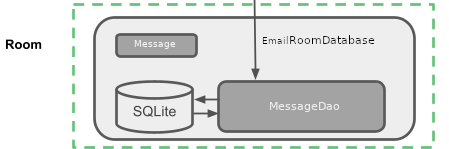
\includegraphics[width=.4\textwidth]{media/RoomStructure.png}
    \caption{Room Struktur \cite{appStructurePicture}}
\end{wrapfigure}



Room ist eine Art Schicht über der SQLite database. 
Room besteht grundsätzlich aus drei Teilen. Die Database dient als Hauptzugriffspunkt für die gespeicherten Daten der App. Sie ist mit @Database markiert. 
Eine \textit{Entity} repräsentiert einen \textit{table} in der Database und die \textit{DAO} Klasse beinhaltet die Methoden, um auf die Database zuzugreifen. Sie kommuniziert
mit SQLite, um den Zugriff auf die Daten zu ermöglichen. \cite{roomStructure}


\paragraph{MessageDao}

In der \textit{DAO}-Klasse können SQL statements verwendet werden. Um auf die Database zuzugreifen und nur Gewisse 
Objekte zu erfassen, braucht es SQL. Mit diesen Codezeilen kann dann nach den \textit{Ordnern} in der Spalte \textit{folder} gesucht werden.
SQL ist in diesem Fall sehr selbsterklärend, 
dennoch werden wir darauf eingehen.\\

\lstset{language=SQL}
\begin{lstlisting}
    /* get Draft messages*/
    @Query("SELECT * FROM message_table WHERE folder LIKE 'Draft' ORDER BY date ASC")
    LiveData<List<Message>> getDraftMessages();
\end{lstlisting}

\textit{Querys} sind Anfragen an die Database nach Informationen. Sie können auf verschiedene \textit{tables} zugreifen und Informationen abgleichen und auswählen. 
In einer DAO von Room werden die SQL-statements mit @Query markiert. SELECT heisst, dass etwas ausgewählt werden soll und mit * ist alles gemeint. Mit FROM wird angegeben von 
welchem table, in diesem Fall vom message\_table. Mit WHERE können Spalten der Entity ausgewählt werden. Hier wird die \textit{folder} Spalte 
gewählt um mit LIKE ein Attribut zu bestimmen. So wird nun ein Attribut namens 'Draft' gewählt. Mit ORDER By kann die Ausgabe noch sortiert werden. So wird die Ausgabe anhand der Spalte 'date'
aufsteigend sortiert. \cite{queryExpl}

Dieses Query wird über das Repository und das Viewmodel, welche gleich erklärt werden, im Fragment Draft ausgeführt. Dieses Fragment wird aufgerufen, wenn der Nutzer 
auf den Ordner Draft drückt. Also ist es so, wenn dieser Ordner aufgerufen wird, wird die Database nach dem Wert 'Draft' im Attribut \textit{folder} abgefragt.

\subsubsection{Repository/ViewModel}

\begingroup
\setlength{\intextsep}{1pt}
\setlength{\columnsep}{4pt}

\begin{wrapfigure}{r}{6.5cm}
    \centering
    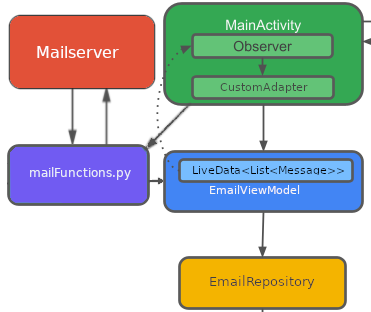
\includegraphics[width=.4\textwidth]{media/RepositoryDataInput.png}
    \caption{EmailViewModel and Repository
    \cite{appStructurePicture}}
\end{wrapfigure}


Damit die Database die Daten einlesen kann, braucht es eine Repository. Über das Repository werden normalerweise Daten aus aller Art von Datenquellen eingelesen. Jedoch
werden in diesem Fall keine Daten vom Server direkt im Repository eingelesen, denn sie gehen zuerst über das Viewmodel.
Weil das Herunterladen der Daten vom Mailserver leider erst sehr spät funktioniert hatte, 
haben sich die Autoren dazu entschlossen, das Einlesen der Daten über das Viewmodel zu machen. Dieses hat eine sehr ähnliche Funktion, 
es leitet die Daten ebenfalls weiter, nur gibt es \gls{livedata} zurück, was dazu führt, dass in der Mainactivity oder im entsprechenden Fragment ein \gls{observer} 
eingebaut werden kann. Dieser informiert die Klasse dann über Veränderungen in der Database, um sie dann

im Recyclerviewer anzeigen zu lassen.
\cite{appStructurePicture}\\


Dies ist die Funktion, welche an einer Variable vom Typ EmailViewModel ausgeführt wird. In dem Fragment 'HomeFragment' in der
onCreateView Funktion, welcher immer ausgeführt wird wenn dieses Fragment aufgerufen wird. 


\lstset{language=java}
\begin{lstlisting}
        mEmailViewModel = new ViewModelProvider(this).get(EmailViewModel.class);
        mEmailViewModel.getInboxMessage().observe(getViewLifecycleOwner(), messages -> {
            /* Update the cached copy of the messages in the adapter*/
            adapter.submitList(messages);
        });
\end{lstlisting}

\begingroup
\nohyphenation

Die Funktion getInboxMessage() ist in der Klasse EmailViewModel und EmailRepository definiert und gibt 

LiveData \textless List \textless Message \textgreater \textgreater  zurück, was soviel ist wie eine Liste der Objekte in der Database, eingebettet 
in LiveData.

\endgroup

\lstset{language=java}
\begin{lstlisting}
    public LiveData<List<Message>> getInboxMessage(){ return mInboxMessage;}

\end{lstlisting}

\lstset{language=java}
\begin{lstlisting}
        private LiveData<List<Message>> mInboxMessage;

        public EmailViewModel(Application application) {
        super(application);
        mEmailRepository = new EmailRepository(application);
        mInboxMessage = mEmailRepository.getInboxMessages();
        }

        public LiveData<List<Message>> getInboxMessage(){ return mInboxMessage;}

\end{lstlisting}

\lstset{language=java}
\begin{lstlisting}
    private LiveData<List<Message>> mInboxMessage;

    public EmailRepository(Application application) {
        EmailRoomDatabase db = EmailRoomDatabase.getDatabase(application);
        messageDao = db.messageDao();
        mInboxMessage = messageDao.getInboxMessages();
    }

        public LiveData<List<Message>> getInboxMessages() {
        return mInboxMessage;
    }


\end{lstlisting}

Es ist ein Schlange, welche sich durch EmialViewModel und EmailRepository zieht. In den beiden \textit{Constructor} wird etwa das gleiche gemacht. Im EmailRepository
werden die Query aus dem MessageDAO ausgeführt, um die Daten in Variablen für jeden Ordner zu speichern. Und im EmailViewModel werden, durch Funktionen aus dem Repository 
die Variablen abgerufen und wieder neu gespeichert, um am Schluss diese Variablen in einem Fragment aufzurufen und dem Adapter gegeben, wie es am Anfang dieser Seite beschrieben 
wird.

\subsubsection{Draft Messages}

\begingroup
\setlength{\intextsep}{5pt}
\setlength{\columnsep}{4pt}

\begin{wrapfigure}{r}{6cm}
    \centering
        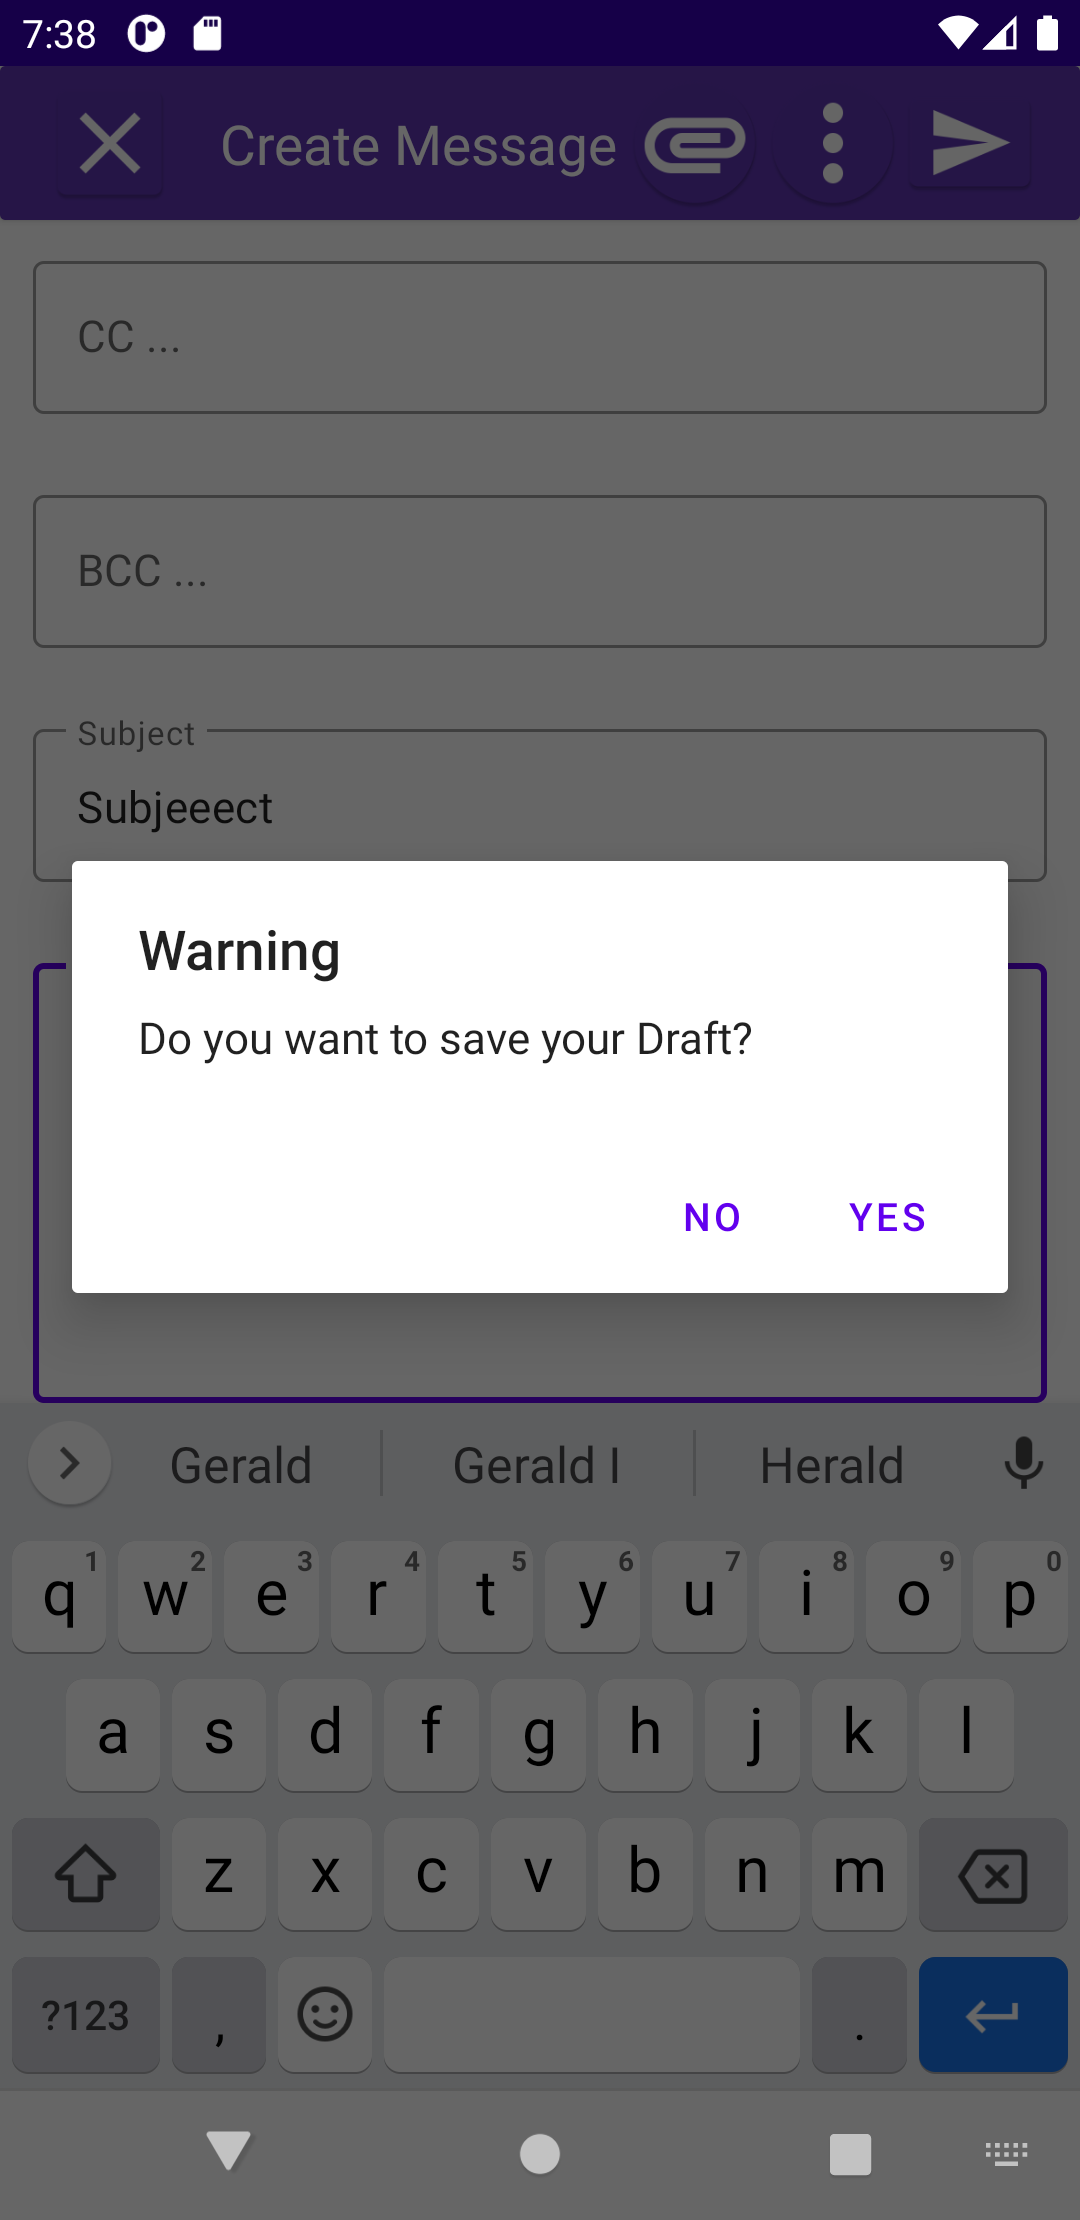
\includegraphics[width=.3\textwidth]{media/EWAttention.png}
        \caption{Email Writer}
\end{wrapfigure}


%\begin{wrapfigure}{r}{9cm}
%    \centering
%    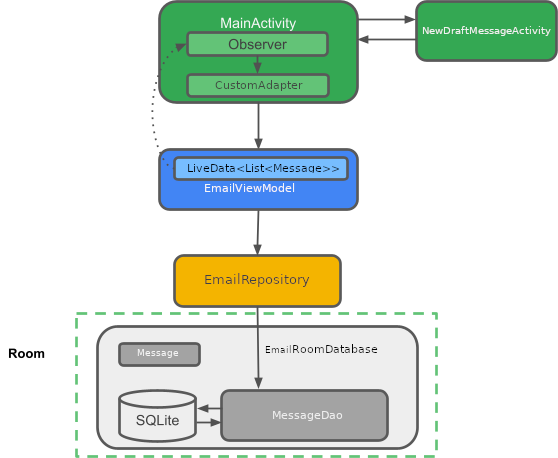
\includegraphics[width=.55\textwidth, height=.55\textwidth]{media/AppStructure.png}
%    \caption{App Structure \cite{appStructurePicture}}
%\end{wrapfigure}

\nohyphenation

Vorhin wurde beschrieben, wie Daten aus der Database ausgelesen werden, wie sie eingelesen werden und wie sie gespeichert werden. Jetzt wird kurz 
noch gezeigt, wann und wie Entwürfe unter dem Namen \say{Drafts} gespeichert werden. \\

Nachdem eine Nachricht geschrieben wurde, kann sie versendet werden oder auch gespeichert werden, wenn im \gls{email writer} das Kreuz gewählt wird, wird der Nutzer 
gefragt, ob er die Nachricht abspeichern möchte. Wenn er die Nachricht speichern will, werden im MessageCreateFragment, welches dem Email Writer entspricht, die
eingegebenen Informationen ausgelesen. Über einen \gls{intent} werden diese Informationen weiter an die MainActivity gesendet und dort 
mit dem \textit{Folder} Attribut \say{Draft} in die Database eingelesen.\\

\endgroup

%TODO: alles um de Server mit Python und repository etc. Dänkfähler mit Aktualisierung vo de Ordner
\vspace*{2cm}
\subsubsection{Server Connection}

\begin{figure}[H]
\center
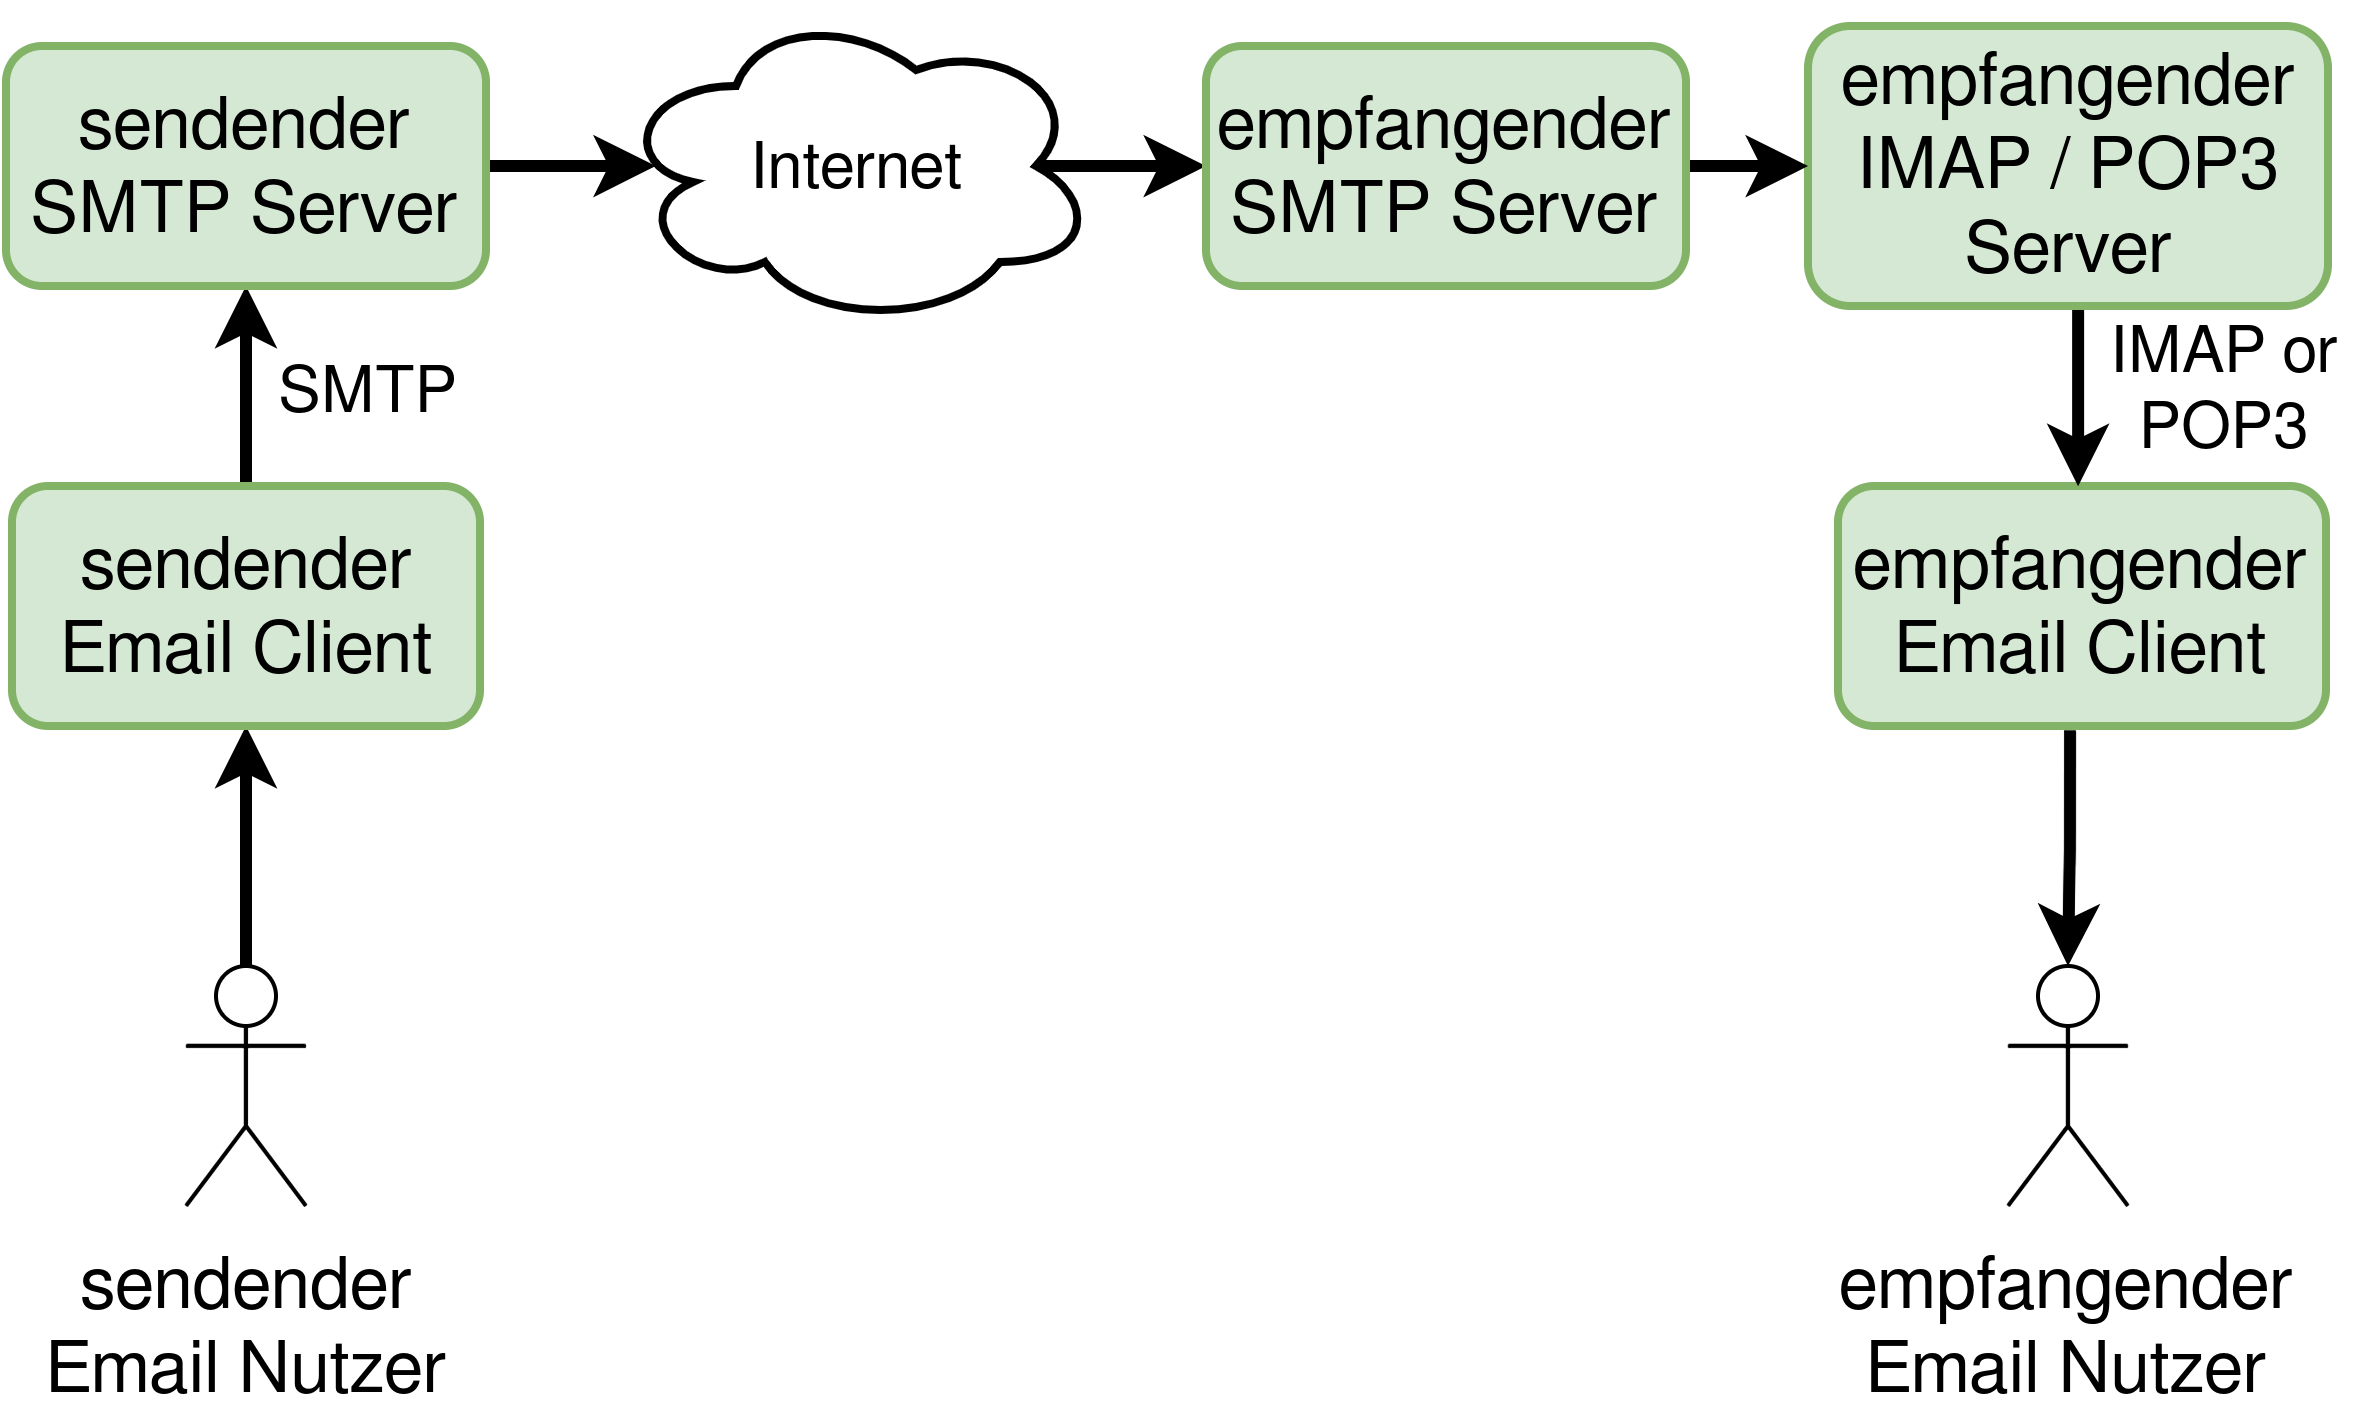
\includegraphics[width=.7\textwidth]{media/connection-diagram.png}
\caption{Diagramm Email Versand}
\end{figure}

\phantom{.} \\ % hack to fix line wrapping in the next paragraph
Vereinfacht funktioniert der Versand von Emails wie im obigen Diagramm: Ein Nutzer, der eine Email versenden will, interagiert mit seinem Mail-Client und gibt durch ihn den Befehl, die Email zu versenden. Der Email Client verschickt die Mail an den SMTP Server des sendenden Nutzers, wo dieser zum SMTP Server des empfangenden Nutzers gelangt, von dort aus zu seinem IMAP oder POP3 Server. Wenn der Mail Client des Empfängers eine Anfrage an seinem SMTP / POP 3 macht, kann er diese einlesen und der Nutzer kann nun seine neue Email lesen.\\

Das Versenden von Mails wird in der App einzeln gemacht: Für jede zu sendende Email wird die Funktion \textit{sendStarttls} (siehe folgend) aufgerufen. Zuerst wird der der \gls{ssl} Kontext initialisiert, dann werden die Angaben der Mail zu einer korrekt kodierten und formatierten Nachricht umgewandelt und schliesslich mit der \textit{smtplib} Bibliothek versendet.

\lstset{language=python}
\begin{lstlisting}
def sendStarttls(host, sendingMail, receivingMail, password, message="",
                 subject="", port=587, cc=[], bcc=[]):
    context = ssl.create_default_context()

    if type(cc) is not str:
        cc = ",".join(cc)
    if type(bcc) is not str:
        bcc = ",".join(bcc)
    utf8Message = ("Subject: " + subject + "\nCC: " + cc + "\nBCC: " + bcc +
                   "\n\n" + message)
    decoded = utf8Message.encode('cp1252').decode('utf-8')

    with smtplib.SMTP(host, port) as serverConnection:
        serverConnection.starttls(context=context)
        serverConnection.login(sendingMail, password)
        serverConnection.sendmail(sendingMail, receivingMail, decoded)
\end{lstlisting}

\subsection{Umsetzung}
\subsubsection{Bugs}
% Erklärung woher, warum falsch, wie gelöst
Programmierfehler schleichen sich in jedem Softwareprojekt ab einer gewissen Komplexitätsstufe ein. Damit hatten auch die Entwickler dieses Projektes zu kämpfen. Hier dazu ein kleines Beispiel:\\

% GUI stuff -> oneliner commit 
Als der RecyclerViewer das erste Mal eingebunden werden konnte, ohne dass die App nach dem Öffnen direkt abstürzte, war das Problem, dass am oberen Teil des UI Inhalte abgeschnitten waren. Das konnte gelöst werden, indem diese Codezeile in der Datei \textit{app/src/main/res/layout/activity\_main.xml} an der richtigen Stelle eingefügt wurde:

\lstset{language=XML}
\begin{lstlisting}
android:paddingTop="50dp"
\end{lstlisting}

Es gab sehr viele Bugs, erst recht gegen Ende der Matur, weil dort erst die meisten Funktionen fertig wurden. 
Ein Bug, der bis Heute nicht gelöst werden konnte, ist das Löschen des \textit{Tables} in der Database. Eigentlich sollte dies eine
Leichtigkeit sein, dennoch war es den Autoren nicht möglich, ein einfaches Room/SQL statement zu finden, welches alle Informationen in der Database löscht. \\

Die Lösung zu diesem Problem hat leider auch einen Haken: Es muss jeder Ordner einmal ausgewählt werden, bevor alle Nachrichten gelöscht werden können. 
Die Lösung an sich war, dass, wenn einer der Ordner geöffnet wird, alle Nachrichten in diesem Ordner in einer Liste gespeichert werden. Wenn dann die Option "Delete all Folder"
gewählt wird, wird ein Loop gestartet, welcher durch die Liste geht und jede Nachricht einzeln ausgibt. Diese Nachricht wird weiter über Umwege an die MessageDAO Klasse gebracht
und dort kann eine einzelne Nachricht gelöscht werden. Es ist eine umständliche Lösung und noch nichteinmal ausgereift. Dennoch besser, als wenn es nicht möglich wäre. \\

Vor kurzer Zeit war dieser Bug noch störender, denn die Nachrichten mussten auch gelöscht werden, wenn ein neuer Account angemeldet wurde. Jedoch 
konnte das umgangen werden, sobald der Account Manager aufkam. Mit diesem mussten die Nachrichten einfach auch nach dem Account abgerufen werden und die Nachrichten
wurden nicht mehr gelöscht. Es wurden einfach nur die Richtigen angezeigt. \\

Die Autoren sind sich ziemlich sicher, dass es weitere Bugs in der App geben wird, da nicht genügend Zeit für das debugging eingeplant . 


\subsubsection{Probleme / Hiccups}
% RecyclerViewer, shit java IMAP libraries
Probleme waren die unnötig vielen Layouts, welche bei der App entstanden sind. Vielleicht hätten diese minimiert werden können, wenn die Entwickler eine signifikant höhere Erfahrung im Bereich der Android Entwicklung gehabt hätten, oder wenn die verschiedenen Inhalte beim Aufrufen weniger Layouts generieren würden, oder diese könnten besser wieder referenziert werden.\\

Mit gewissen Bibliotheken sind auch Probleme entstanden, dazu wird später in diesem Text noch das Problem mit den Email-Bibliotheken geschildert.

\subsubsection{Kommunikation}

Die Menge an Kommunikation hat sich eingependelt zwischen den Anforderungen, Bedürfnissen und sozialen Kapazitäten der beiden Autoren. Einer wollte eher etwas mehr Dialog, der andere weniger. Das gegenseitige Vertrauen war aber auch soweit vorhanden, dass man sicher sein konnte, dass der andere gewisse abgemachte Zeiten einhält und Nachrichten nicht unnötig lange unbeantwortet lässt.\\

Es konnten auch gute Strukturen für die Kommunikation geschaffen werden, so wurde eine \textit{diary}, also eine Art Tage- oder Logbuch verwendet, um den Arbeitsprozess zu dokumentieren, was sich insbesondere bei den Anfängen des Projektes als nützlich herausstellte. Auf diesem Dokument und der \textit{Git Commit History} basiert die Dokumentation dieser Arbeit.\\

Sowohl im Programm-Quellcode der App als auch im Quellcode dieser Arbeit haben die beiden Autoren Notizen in Form von Codekommentaren gemacht - teilweise sich sogar gegenseitig- voll nach dem Motto: \say{Hey, kannst du das dann dort noch einfügen? Du kannst das ja besser als ich.}\\

Auch haben sich die beiden zeitweise Montags zusammen hingesetzt um den Arbeitsprozess in dieser Weise zu besprechen und um die nächsten Aufgaben zu verteilen.\\

Insgesamt verlief die Kommunikation doch reichhaltig, obwohl einer der beiden Autoren doch etwas überdurch-schnittlich schwer digital erreichbar ist. Die grobe Aufteilung des Programmes, um daran zu entwickeln und die Komponenten wieder zusammenzufügen, hatte etwas von der typischen Modularität von Linux.
% TODO: bruche mir de satz mit de 'linuxphilosophie' @simon? weiss grad iwie nid. Doch ich find dä super

\subsubsection{Namensfindung}
Für die App musste auch noch ein Name her, doch die aller längste Zeit hatten die beiden Autoren entweder keine Idee oder der Name wurde schon von einer anderen App verwendet. Doch als einer der beiden Autoren seinen Vater nach Namensideen fragte, war einer der Vorschläge \say{Schneckenpost}. Dies ist natürlich eine offensichtliche ironische Anspielung darauf, dass unsere App schneller sein soll als die meisten Apps. Doch da ein englischer Name erwünscht war, wurde es einfach direkt übersetzt in \say{snail mail}. Nun war nur noch die Frage, wie man es darstellen sollte, etwa \say{SnailMail} (CamelCase), \say{snailMail} (mixedCase), \say{Snail Mail}, \say{snail mail} oder \say{snailmail}. Es wurde für das Letzteres entschieden, da dies das wichtigste Designkonzept der App am besten widerspiegelt: Die Einfachheit. Gleich wie die App lautet auch übrigens der Name des GitHub Repositorys der App:\\

\url{https://github.com/noahvogt/snailmail}

\subsection{Testing}

Zum Testen gibt es soweit nicht sehr viel zu sagen, da die Autoren fortlaufend das Programm ausprobiert haben und die Resultate direkt wieder in das Programm flossen.
Es hätte keinen Mehrwert gehabt, die \say{Ergebnisse} solcher einfachen Tests zu dokumentieren. Wofür die Zeit leider nicht gereicht hat, war das 
richtige Testen der App im Alltag. Da die App noch nicht fertig ist und die neuste Version auch erst vor Kurzem entstand, konnte die App nicht an Bekannte gegeben werden
und ein paar Tage getestet werden. Das Interface wurde zwar getestet aber darüber hinaus leider nicht viel.

\section{Resultate}
\subsection{Vergleich mit unseren ursprünglichen Zielen}
Das User Interface ist erfreulich gut im Einklang mit den ursprünglichen Zielen; es ist wirklich einfach ohne irgendwelchen unnötigen Schnickschnack. Simpel ist das GUI also, doch wie steht es mit der Bedienerfreundlichkeit? Dazu haben wir Freunde und Bekannte eingespannt, ihnen ein Handy mit der App in die Hand gedrückt und gesagt, sie sollen einen Mail Account einrichten, um dies herauszufinden. Dabei haben sich die meisten gut und schnell zurechtgefunden, obwohl die App ja noch nicht fertig ist.\\

Die App selber ist wie von uns in den Zielen vorgegeben Free Software. Doch erst kürzlich kam auf, dass die von diesem Projekt verwendete \say{chaquopy} Bibliothek proprietär ist, und somit indirekt ein Konflikt mit den ursprünglichen Zielen steht: Es wurde zwar nicht explizit angegeben, dass alle Bibliotheken zwingend auch Open Source sein sollen, doch es ist nicht im Sinne der Autoren eine nichtfreie Library zu verwenden. Im Laufe der weiteren Softwareentwicklung wird dieser Fehler noch unbedingt behoben werden müssen. Dieser Missstand ist auch teilweise dem Dependencymanagement von Gradle anzulasten, da dieser immer nur die binäre Version herunterlädt und der Source Code von Dependencies nirgends gescheit verlinkt ist.\\

%TODO @noah glossar -> HTML Output parsing -> not mentioned
Die wichtigsten Funktionen der App wurden erreicht, es können Emails geschrieben, gelesen werden, es bestehen verschiedene Mailboxen und jeder kann seine Email Accounts gut managen, also hinzufügen, ändern und entfernen. Gewisse Features, wie Pushnachrichten, Suchfunktionen, ein visuelles Attribut, wo zu sehen ist, ob eine Nachricht gelesen wurde, fehlen noch ganz. Funktionen wie die Einstellungen, das synchronisieren der Datenbank mit dem Mailserver und die Anhang Funktionalität sind noch nicht fertiggestellt. Es gibt auch noch gewisse Bugs bei der Entstehung von \say{edge cases} \cite{edgecase} bei bestimmten einzelnen Emails.\\

Ursprünglich wurde zusätzlich ein Pluginmanager - dabei angelehnt an die Funktionsweise von vim-plug \cite{plug} - geplant einzubauen, doch diese Idee wurde mittlerweile verworfen, da es weitaus sinnvoller und effizienter von den Autoren angesehen wurde, einfach klassische Patches zu verwenden. Ähnlich wie dies bei der suckless.org Software ist. \cite{dwm}

\subsection{Vergleich mit der Konkurrenz}
Es ist gar nicht so einfach, diese App zu vergleichen mit ihrer Konkurrenz, da sie noch nicht fertig entwickelt ist. Aus diesem Standpunkt heraus vergleichen wir nur die fertigen Funktionen mit der Konkurrenz.\\

Im Vergleich mit der Konkurrenz sticht die App heraus durch ihre simple Art, so wie das geplant war. Die Funktionalitäten sind dabei auch wesentlich rudimentärer, oder besser gesagt, mehr \say{suckless}, als die der Konkurrenz. Die Farben und das Layout des User Interface sollte zwar simpel sein, doch das visuelle Zusammenspielen von Farben und dem Layout haben gewisse Konkurrenzprodukte, welche immerhin auch von Fortune 500 Unternehmen entwickelt werden, zweifelsohne besser umgesetzt, als die Autoren dieser App.
\subsection{Vor- und Nachteile unserer App}
\subsubsection{Pro}
Für die Nutzung der App sprechen simple Nutzeroberfläche und Codebasis, welche nach Fertigstellung der initialen Entwicklung einer der besten simplen Email-Clients werden kann.

\subsubsection{Kontra}
Dagegen sprechen, dass gewisse Funktionen, welche laut den Autoren nicht in einen Email-Client gehören, nicht vorhanden sind, wie beispielsweise die Funktionalität eines eingebauten Kalenders, wie es der allseits bekannte Mailclient Thunderbird zu tun pflegt.\cite{thunderbird}

\section{Selbstreflexion}

\subsection{Was Gut Lief}
% komm., vcs, java syntax (allg.)
Das Arbeiten mit \textit{Git} als \textit{Version Control System} verlief gut und half enorm beim Arbeitsprozess und dessen Strukturierung. Mit der Syntax der verwendeten Programmier- und Markupsprachen Java, Python und XML konnte gut umgegangen werden, obwohl die beiden noch recht wenig Erfahrung mit Java hatten. Die Codestruktur fanden sie den Umständen entsprechen gut und sinnvoll.
\subsection{Was Schlecht Lief}
Es gab keine mit Gradle funktionierende, ausreichend dokumentierte und/oder nicht veraltete IMAP- und Email Bibliotheken für Java. Deshalb wichen wir auf die um Welten besser funktionierende Python Bibliotheken \textit{imap} und \textit{emaillib} aus. Dazu mussten wir eine Library namens \textit{chaquopy} benutzen, um Python als Bytecode kompiliert in unsere Java App einbauen zu können. Das ist natürlich unschön, aber die Funktionalität hatte die oberste Priorität.\\

%TODO: wir person
Etwas, das nicht direkt schlecht lief, aber sehr viel Zeit raubte ist, dass wenn einer der Autoren zum Beispiel eine Database für den Recyclerviewer gemacht hatte, zwar nur eine Testversion, 
er diese im späteren Verlauf komplett überarbeiten durfte. Es war zwar nur eine Testversion, aber, dass diese so weit von einer professionelle Database entfernt war, war ihm nicht klar. 
In so einer Situation war er nicht nur bei der Database. Mit dem Recyclerviewer hatte er solche Probleme sogar öfters. Oft hat zwar noch nicht viel funktioniert, aber er musste den Recyclerviewer
mehrmals komplett umschreiben. \\


%TODO:@Noah dinni Meinig dezue? -> erklären
Etwas, das sicher hätte besser laufen sollen, war das Zeitmanagement. Wir hatten zwar mögliche Komplikationen miteinberechnet im Zeitplan, doch wir hatten viel mehr und verheerendere Probleme, welche unseren Zeitplan regelrecht herausforderten, schlisslich waren wir beinahe immer in Zeitverzug. Im Sommer dachten wir noch, wir wären perfekt in der Zeit und dies wurde uns auch bestätigt. Jedoch
als wir aus den Sommerferien kamen, wurde uns bewusst, wie viel es noch zu tun gab. Wir haben alles gegeben, jedoch wurde die App leider nicht fertig. 

\subsection{Was Wir Gleich Machen Würden}
Wenn wir in die Vergangenheit reisen und die App von Neuem machen könnten, würden wir am User Design nichts ändern, und auch weiterhin mit \textit{Git} als \textit{VCS} arbeiten und für jedes noch nicht einsatzbereite Feature einen neuen \textit{Branch} machen. Die Arbeitsweise an sich hat sich aus unserer Sicht bewährt und ist ein passabler Weg, kollaborativ an einem Softwareprojekt zu arbeiten.


\subsection{Was Wir Anders Machen Würden}

Der Code, der in Java geschrieben wurde, kann nicht nativ auf einer Maschine laufen, sondern muss durch eine virtuelle Maschine, die \textit{Java Virtual Machine (JVM)} während der Ausführung in nativen Code umgewandelt werden. Deshalb würde bei einem Rewrite wohl besser mehr Code in C oder C++ geschrieben werden, um die Geschwindigkeit und Portabilität zu erhöhen. Java komplett wegzulassen, ist weder vorgesehen, noch praktisch sinnvoll umsetzbar. \\

Uns ist öfters gesagt worden, dass das Managen der Zeit sehr wichtig ist. Wir sind davon ausgegangen, dass wir diese auch gut eingeplant hatten. Dem war leider nicht so und wir 
würden uns mehr Gedanken machen beim Planen, wie auch, wie lange wir an einem Problem arbeiten, bevor wir das Feature entfernen, als dass wir sehr lange daran arbeiten. 


\subsection{Abschliessende Persönliche Schlussfolgerung}
Wir haben das Gefühl, einen guten ersten Einblick in die native Android Programmierung mit Java und Python bekommen zu haben. Wir haben uns vertraut gemacht mit den Vorzügen, aber auch Nachteilen dieser Art von Programmierung und der Plattform Android.\\

Wir sind zwar etwas enttäuscht, dass wir nicht alle geplanten Ziele erreicht haben, doch wir haben noch genug Motivation, die App in den nächsten paar Wochen und Monaten fertigzustellen. Denn die Arbeit hat uns insgesamt doch gefallen, trotz einigen Motivationstiefs, sodass wir auch gerne unseren Freunden und Familien von ihr erzählt haben.
Wir können sicher sagen, dass wir jetzt eine Smartphone App als grösseres Projekt ansehen als das, was wir dachten. Eine App ist nicht so simpel wie wir erwartet haben.\\

Was uns auch noch sehr gefallen hat, ist das Arbeiten mit dem Version Control System \textit{Git} und der Plattform \textit{Github}, denn so konnte man gut den Fortschritt sehen und tracken, schliesslich machte das kollaborative Arbeiten an einem Projekt dieser Grösse besonders Sinn und konnte gut Nutzen machen von der Funktionalität dieses Systems.
Dazu war das eine sehr gute Lehre wie später in grösseren Teams solche Programme entstehen. Wir sind jetzt sicher etwas besser ausgerüstet als andere.

\section{Danksagung}
Wir - Simon und Noah - möchten uns bei unserer Betreuungslehrperson Dr. Viktor Yakonthov, und unserem Koreferenten D. Bühler bedanken, dass sie uns die Arbeit haben durchführen lassen und ihre Bereitschaft gezeigt haben, bei allfälligen Fragen zu helfen.\\

Ein besonderer Dank gilt auch unseren beiden Müttern, welche den Text durchgelesen haben und versucht haben, unsere sprachlichen Fehler zu korrigieren. Ausserdem möchten wir uns noch bei Noahs Vater bedanken, welcher uns die Namenidee für unsere App gab.

\clearpage
\printglossary

\newpage
\printbibliography[heading=bibnumbered, title={Literaturverzeichnis}]

\listoffigures

\newpage
\begin{appendices}
\subsection*{Open-Source Programme}
Es wurden Open-Source Programme genutzt um verschiedene Elemente einbauen zu können. 

Für die Library Room haben sich die Autoren an diesem Programm bedient. \cite{roomApp}
Stark betroffen sind die Dateien \textit{EmailViewModel.java}, \textit{EmailViewHolder.java}, \textit{CustomAdapter.java}, \textit{EmailRepository.java}, \textit{EmailRoomDatabase.java}, \textit{Message.java}, \textit{MessageDao.java}
und \textit{NewDraftMessageActivity.java}. Bei diesen
Dateien handelt es sich um Templates, sie wurden stark erweitert und dazu werden sie von anderen Funktionen aufgerufen. 
Die Dateien von denen sie inspiriert wurden, heissen fast gleich. Es muss nur \say{Email} und \say{Message} durch \say{Word} ersetzt werden und Sie finden die Dateien.
Die Dateien \textit{ArchiveFragment.java}, \textit{GalleryFragment.java}, \textit{HomeFragment.java}, \textit{DraftFragment.java}, \textit{SpamFragment.java} und \textit{MainActivity.java} beinhalten alle vier Zeilen beginnend mit der 
Variabel \say{mEmailViewModel} vom Typ \say{EmailViewModel}. Diese vier Zeilen sind jeweils auch aus dem Basisprogramm. 
Die Zeilen sehen etwa so aus:
\lstset{language=java}
\begin{lstlisting}
    mEmailViewModel = new ViewModelProvider(this).get(EmailViewModel.class);
    mEmailViewModel.getArchiveMessage().observe(getViewLifecycleOwner(), messages -> {
        /* Update the cached copy of the messages in the adapter*/
        adapter.submitList(messages);

\end{lstlisting}


Weiter beinhaltet die Datei \textit{MainActivity.java} eine Funktion namens \say{onActivityResult}, welche auch aus dem Basisprogramm stammt. 
    \lstset{language=java}
    \begin{lstlisting}
    public void onActivityResult(int requestCode, int resultCode, Intent data) {
        super.onActivityResult(requestCode, resultCode, data);

        if (requestCode == NEW_WORD_ACTIVITY_REQUEST_CODE && resultCode == RESULT_OK) {
            Word word = new Word(data.getStringExtra(NewWordActivity.EXTRA_REPLY));
            mWordViewModel.insert(word);
        } else {
            Toast.makeText(
                    getApplicationContext(),
                    R.string.empty_not_saved,
                    Toast.LENGTH_LONG).show();
        }
    }
    \end{lstlisting}
Diese Zeilen waren Grundlage für die nachfolgenden Zeilen.

\lstset{language=java}
\begin{lstlisting}
 public void onActivityResult(int requestCode, int resultCode, Intent data) {
            super.onActivityResult(requestCode, resultCode, MessageCreateFragment.replyIntent);

        /* Creates class for the Date when Email is written */
        Date dNow = new Date();
        SimpleDateFormat ft =
                new SimpleDateFormat("dd.MM.yy");
        System.out.println(dNow);

            Message word = new Message(userGlobal,
                MessageCreateFragment.replyIntent.getStringExtra(MessageCreateFragment.EXTRA_TO),
                MessageCreateFragment.replyIntent.getStringExtra(MessageCreateFragment.EXTRA_CC),
                MessageCreateFragment.replyIntent.getStringExtra(MessageCreateFragment.EXTRA_BCC),
                MessageCreateFragment.replyIntent.getStringExtra(MessageCreateFragment.EXTRA_FROM),
                ft.format(dNow),
                MessageCreateFragment.replyIntent.getStringExtra(MessageCreateFragment.EXTRA_SUBJECT),
                MessageCreateFragment.replyIntent.getStringExtra(MessageCreateFragment.EXTRA_MESSAGE),
                "Draft",false);
            mEmailViewModel.insert(word);
        }
\end{lstlisting}

Sehr ähnliche Zeilen befinden sich auch in der \textit{messageCreateFragment.java} Datei von Zeile 150-171. Diese stammen ursprünglich auch aus dem Basisprogramm, 
wurden aber überarbeitet. 

\lstset{language=java}
\begin{lstlisting}
final Button button = findViewById(R.id.button_save);
        button.setOnClickListener(view -> {
            Intent replyIntent = new Intent();
            if (TextUtils.isEmpty(mEditWordView.getText())) {
                setResult(RESULT_CANCELED, replyIntent);
            } else {
                String word = mEditWordView.getText().toString();
                replyIntent.putExtra(EXTRA_REPLY, word);
                setResult(RESULT_OK, replyIntent);
            }
            finish();
        });
\end{lstlisting}

Diese Zeilen waren Grundlagen für die nachfolgenden Zeilen.

\lstset{language=java}
\begin{lstlisting}
activity.setResult(RESULT_CANCELED, replyIntent);

    String from = sendingAddressObject.getText().toString();
    String to = receivingAddressObject.getText().toString();
    String subject = subjectObject.getText().toString();
    String message = messageBodyObject.getText().toString();
    String cc = ccObject.getText().toString();
    String bcc = bccObject.getText().toString();


    replyIntent.putExtra(EXTRA_FROM, from);
    replyIntent.putExtra(EXTRA_TO, to);
    replyIntent.putExtra(EXTRA_CC, cc);
    replyIntent.putExtra(EXTRA_BCC, bcc);
    replyIntent.putExtra(EXTRA_SUBJECT, subject);
    replyIntent.putExtra(EXTRA_MESSAGE, message);
    activity.setResult(RESULT_OK, replyIntent);

    activity.finish();

        Intent intent = new Intent(getContext(), NewDraftMessageActivity.class);
        startActivityForResult(intent, MainActivity.NEW_WORD_ACTIVITY_REQUEST_CODE);

\end{lstlisting}

\end{appendices}


\end{document}
